\documentclass{book}

% Language setting
% Replace `english' with e.g. `spanish' to change the document language
\usepackage[english]{babel}

% Set page size and margins
% Replace `letterpaper' with `a4paper' for UK/EU standard size
\usepackage[letterpaper,top=2cm,bottom=2cm,left=3cm,right=3cm,marginparwidth=1.75cm]{geometry}
\usepackage{color}

% Useful packages
\usepackage{amsmath,amsfonts,amssymb}
\usepackage{amsthm}
\usepackage[colorlinks=true, allcolors=blue]{hyperref}
\usepackage{hyperref}
\usepackage{graphicx}
\usepackage{caption}
\usepackage{subcaption}
\graphicspath{ {figs/} }



% for crossing out math terms in derivations
\usepackage{cancel}

\usepackage[printsolution=false]{exercises}


% Define theorem like objects
\newtheorem{theorem}{Theorem}
\newtheorem{lemma}{Lemma}

\usepackage{mathtools}
\mathtoolsset{showonlyrefs}

\newcommand{\e}{\varepsilon}
\newcommand{\dx}{\, dx}
\newcommand{\dt}{\, dt}
\newcommand{\ds}{\, ds}
\newcommand{\dy}{\, dy}
\newcommand{\dz}{\, dz}
\newcommand{\dr}{\, dr}
\newcommand{\dw}{\, dw}
\newcommand{\x}{{ \bf x}}
\newcommand{\w}{{ \bf w}}
\newcommand{\y}{{\bf y}}
\newcommand{\al}{\alpha}
\newcommand{\R}{\mathbb{R}}
\newcommand{\N}{\mathbb{N}}
\newcommand{\E}{\mathbb{E}}
\newcommand{\HH}{\mathcal{H}}
\DeclareMathOperator{\Prob}{\mathbb{P}}
\renewcommand{\P}{\mathbb{P}}
\newcommand{\M}{\mathcal{M}}
\renewcommand{\div}{\text{div}\,}
\newcommand{\sym}{\text{sym}}
\newcommand{\diam}{\textup{diam}\,}
\newcommand{\grad}{\nabla}
\newcommand{\lambdaMin}{\lambda_{\textup{min}}}
\newcommand{\lambdaMax}{\lambda_{\textup{max}}}
\newcommand{\vxavg}{\vx_{\textup{avg}}}
\newcommand{\xavg}{x_{\textup{avg}}}
\newcommand{\xperp}{x_{nc}}
\newcommand{\vxperp}{\vx_{nc}}
\newcommand{\ones}{{\bf 1}}
\newcommand{\myDiag}{\textup{diag}\,}
\newcommand{\ddt}{\frac{d}{dt}}
\newcommand{\cl}{\textup{cl}}
\newcommand{\dtau}{\,d\tau}
\newcommand{\myspan}{\textup{span}}
\newcommand{\Var}{\textup{Var}}
%\newcommand{\C}{\mathfrak{C}}
\newcommand{\C}{\mathcal{C}}
\newcommand{\cons}{\mathfrak{C}}
\newcommand{\vecc}{\text{vecc}}
\newcommand{\diag}{\text{diag}}
\newcommand{\ns}{{n_s}}
\newcommand{\Proj}{\textup{P}}
\newcommand{\Hess}{\nabla^2}
\newcommand{\myrank}{\textup{rank}\,}
\newcommand{\ELBO}{\text{ELBO}}
\newcommand{\calL}{\mathcal{L}}
\newcommand{\calF}{\mathcal{F}}
\newcommand{\eps}{\varepsilon}
\newcommand{\col}{\text{col}\,}
\newcommand{\row}{\text{row}\,}
\newcommand{\calN}{\mathcal{N}}
\newcommand{\calD}{\mathcal{D}}


% Transpose symbol
\makeatletter
\newcommand*{\T}{%
  {\mathpalette\@T{}} %
}
\newcommand*{\@T}[1]{
  \raisebox{\depth}{$\m@th#1\intercal$}%
}
\makeatother


\def\myred#1{\textbf{\textcolor{red}{#1}}}

\title{Personal Notes}
\author{}
\date{}

\begin{document}
\maketitle

\tableofcontents


\include{lin-algebra-chap}

\chapter{Calculus and Analysis For Machine Learning}

Possible sections:
\begin{itemize}
  \item Some basic calculus results (MVT, extreme value theorem, etc.) 
  \item Fundamental theorem of calculus (then, implications? Like, how is this useful for...)
  \item Inverse and implicit function theorems (and implications) 
  \item Divergence theorem (and relationship to fundamental theorem of calculus)
  \item Stokes theorem? (Does this apply to higher than $\R^3$?) 
  \item integration by parts (and some implications. Like for ML?) 
  \item Multivariable chain rule
  \item Change of variables theorem
\end{itemize}


\chapter{Least Squares and Linear Regression}
\section{Least Squares: Linear Algebra Perspective} 
Let
$$
\x_i \in \R^m,\quad y_i \in \R, \quad\quad i=1,\ldots, m.
$$

\vspace{1em}
Here, we have $m$ examples where $x_i$ is a feature vector and $y_i$ is a label. 
Let
$$
X = 
\begin{pmatrix}
    -x_1-\\
    \vdots\\
    -x_m-
\end{pmatrix}\in \R^{m\times n}
\quad \quad \quad
\y = 
\begin{pmatrix}
    y_1\\
    \vdots\\
    y_m
\end{pmatrix} \in \R^{n}
$$

The matrix $X$ is commonly known as the design matrix. We wish to solve 
\begin{equation} \label{eq:least-squares}
X\hat \w = \y. 
\end{equation}

In typical least squares applications, we have $m > n$. This means we have an overdetermined system---there are more equations than variables. We'll deal with that case first, then we'll consider connections to the pseudo inverse. Then we'll consider the complementary case where $m<n$ to complete the picture. 


\subsection{Standard Least Squares: $m>n$} \label{sec:least-squares1}
Note that $X$ is tall and $\dim \col X \leq n < m$. The nullspace $N(X)$ may or may not be empty.  if we assume $\myrank X = n$, then 
  \begin{itemize}
    \item $X$ has linearly independent columns
    \item $\dim \col X = n$
    \item $N(X) = \{0\}$ (by rank-nullity theorem)
  \end{itemize}
We'll assume $\myrank X = n$. Suppose for now that $\hat y\in \col X$. There exists a unique $\hat w$ solving $X\hat w = \hat y$ (see Exercise \ref{exer:restricted-bijection}). 
Now, suppose $y$ may not lie in $\col X$. We would like to find $\hat w$ such that 
\begin{equation} \label{eq:LSQ-opt-prob}
\hat w \in \arg\min_{w} \|Xw - y\|_2^2.
\end{equation}
(Hence the name ``least squares solution.'')
We're in a Hilbert space, so this is just the projection of $y$ onto $\col X$. In particular, the projection theorem (recall it?) gives us existence and uniqueness of a solution. Hence, the optimal $\hat w$ satisfies $(X\hat w- y) \perp \col X$. Equivalently, $(X\hat w - y)^\T X = 0 \iff \hat{w}^\T X^\T X = \y^\T X \iff X^\T X \hat w = X^\T \y$. We know that $(X^\T X)^{-1}$ exists, hence our least squares solution is
\begin{equation} \label{eq:LS-soln1}
\hat w = (X^\T X)X^\T\y.
\end{equation} 
Critically, this is the least squares solution of \eqref{eq:least-squares} when $X$ is tall and full rank. We will treat the case when $X$ is fat in the next section. In Section  \ref{sec:LSQ-pseudo-inv} we will see that both of these cases can be seamlessly handled by applying the pseudo-inverse. 



%\myred{Comment}: This is a nice exposition and all. But it feels kind of long and meandering. The pseudo inverse cuts right to the chase. Should I really just present it that way, and then have this as some kind of supporting material in case one wants to look at from a different perspective and get a little more insight. I'm more interested in remembering that the solution is the pseudo inverse, remembering the form of the pseudo inverse when $X$ is full column rank, and knowing efficient/effective ways to compute it in practice. Though, actually, since I often expect we'll be in the full column rank setting, this is kind of nice to see. And it's not that long, really. 

\subsection{Other case: $m<n$}

In Section \ref{sec:least-squares1} we could not solve \eqref{eq:least-squares} because $X$ was tall and the system was overdetermined. No solution existed.\footnote{If $\myrank X\in \R^{m\times n}$ were less than $n$, then $N(X)$ would be nonempty and a solution would exist.} In this section, we treat the case where $X$ is fat. The system is underdetermined. We have few equations and many unknowns. And $N(X)$ is necessarily nonempty. 

Editorial comment: I get why you care about the $X$ tall case. But why do we care about solving the $X$ fat case in practice? 

To make life easier, assume for now that $\myrank X = m$. Then $\dim \col X = m$. Viewed as a linear transformation, $X$ is surjective and $y\in \col X$. Since $N(X) \not= \{0\}$, there exists many solutions to \eqref{eq:least-squares}. How can we narrow down the set of solutions and pick one? Some options:
\begin{itemize}
    \item Pick $\hat w$ so $\|\hat w\|_2$ is small
    \item Pick sparsest $w$---i.e., so $\|w\|_0$ is small
\end{itemize}
The first idea jives with the notion of regularization and picking a "low complexity" solution. The second is related to compressed sensing and LASSO. 

For now, we'll go with option 1. Suppose $\hat w$ and $w$ both solve \eqref{eq:least-squares}. Then $\hat w - w \in N(X)$. If $\hat w$ lies in the rowspace of $X$ then $\hat w \perp (\hat w - w)$, since $\row X \perp N(x)$. Suppose $\hat w \not = w$. Then
\begin{align}
  \|\hat w\|^2 & = \langle w + (\hat w - w), w + (\hat w - w)  \rangle\\
  & \|w\|^2 - \|\hat w - w\|^2 > \|w\|^2.
\end{align}
Hence, if there exists a solution in the rowspace, it has minimum norm and is unique. 

Recall that the transformation $X$ may be viewed as a bijection between $\col X$ and $\row X$ (e.g., see Exercise \ref{exer:restricted-bijection}). Since $y \in \col X$, and the solution we're looking for is $\hat w \in \row X$, we may recover $\hat w$ if we can compute the inverse of our bijective map restricted to these sets. This is precisely what the pseudo inverse does, as discussed in Section \ref{sec:LSQ-pseudo-inv}. 

For now, we take a slightly more hands on approach to demonstrate an alternative and maybe more illustrative way to arrive at the solution when $X$ is full rank. Note that $\myrank X = \myrank X^\T X = \myrank X X^\T = \myrank X X^\T$ (see Exercise \ref{exer:rank-eqs}). 
Since we assumed $\myrank X = m$ ($X$ fat), we get $\myrank X X^\T = m \iff (X X^\T)^{-1}$ exists. We want to solve \eqref{eq:least-squares}. Anything we can set $\hat w$ to to make this work? 
Let 
\begin{equation}\label{eq:LS-soln2}
\hat \w = X^\T (X X^\T)^{-1}\y.
\end{equation}
Then $X\hat w = XX^\T (X X^\T)^{-1} y = y$. 
Note that if we let $z = (XX^\T)^{-1}\y$, then $\hat \w = X^\T z$, hence $\hat \w \in \row X$. 
Hence, $\hat \w$ is our unique rowspace solution to \eqref{eq:least-squares}. 

In Section \ref{sec:LSQ-pseudo-inv} we'll use the pseudo inverse to generalize this to handle the rank-deficient case and tie it together with the tall $X$ case of Section \eqref{sec:least-squares1}.


\subsection{Least Squares and the Pseudo Inverse} \label{sec:LSQ-pseudo-inv}
A linear mapping $A$ is a bijection from $\row A$ to $\col A$ (see Exercise \ref{exer:restricted-bijection}). The pseudo inverse, studied in Section \ref{sec:pseudo-inv}, gives the inverse map from $\col A$ to $\row A$. It maps $\col A^{\perp} = N(A^\T)$ to zero. This is the exact operation we required when deriving the solutions to \eqref{eq:least-squares} when $X$ was tall and fat in \eqref{eq:LS-soln1} and \eqref{eq:LS-soln2} respectively. The pseudo-inverse generalizes these in the sense that 
$$
\hat \w = X^+\y
$$
is identical to \eqref{eq:LS-soln1} and \eqref{eq:LS-soln2}  in the cases previously studied. Moreover, the pseudo inverse applies more generally and gives the solution to \eqref{eq:least-squares} when is $X$ is tall or fat and when $X$ is rank deficient. 

\section{Gauss-Markov Theorem: Least Squares and MLE} \label{sec:Gauss-Markov}
\myred{TODO} Connect that MLE is optimal estimator in some sense in presence of gaussian noise

\section{Ridge Regression}
\myred{TODO} Set up ridge regression. Explain it in terms of regularization. (Maybe see Tibshirani notes about why shrinking coefficients is helpful.) Also, connect to improving the condition number/stability of the pseudo inverse. Add a numerical example. Also,...\\

Ridge regression uses the following estimator instead of the pseudo inverse \myred{TODO} Add eqref to psudo inverse section. 
\begin{equation} \label{eq:ridge-regression}
\hat w = (X^\T X + \lambda I)^{-1}X^\T\y.
\end{equation}
This can be helpful for improving numerical stability when $X$ has many rows that are almost colinear (so $X^\T X$ is ill conditioned). That was supposedly the original motivation. It can also be helpful for regularization in terms of restricting the hypothesis class. I need to do some work to understand better why this is. But it seems to be generally helpful up to a point. Also, it can be interpreted as a formulation of optimizing \eqref{eq:LSQ-opt-prob} with $\w$ restricted to a ball of a given radius. (You interpret this as optimizing the Lagrangian of that problem, or something like that.) 

\section{LASSO and Elastic Nets}
\myred{TODO}: Add sections about these? To paint a more complete picture? Maybe just keep them really short for now so I remember they're relevant and what people claim about them?



\section{Bayesian Linear Regression}
Let $\w\in \R^n$ and consider the standard linear regression model with Gaussian noise
$$
f(\x) = \x^\T \w, \quad\quad y = f(\x) + \eps
$$
where $\eps \sim \calN(0, \sigma_n^2)$. Here $\x \in \R^n$ denotes a vector of covariates, $y$ denotes a scalar output, and $\calD = \{(\x_i, y_i),i=1,\ldots,m \}$ denotes our data set of $m$ observations. All outputs are assumed to be independent, and we make no assumptions about the distribution of inputs. Let the column vectors $\x_i$ for all inputs be aggregated in the $n \times m$ matrix $X$.\footnote{In stats literature the matrix $X^\T$ is typically referred to as the design matrix. Rasmussen uses the transpose of this.} In the non-Bayesian settings discussed previously, our goal was to come up with a point estimate of $\w$. In the Bayesian setting, we will assume a prior 
$$
\w\sim \mathcal{N}(0, \Sigma_p).
$$

\noindent
\textbf{Goals}: Having a prior, we may compute a couple of important things that are impossible in the previous settings. We are going to try and compute the posterior distribution on $\w$
\begin{equation} \label{eq:BLR-goal}
p(\w|X, \y) \hspace{2em}
\end{equation}
and the posterior predictive distribution 
$$
p(f_*|\x_*, X, \y)
$$
The first term is the distribution of $\w$ conditioned on our observed data $\calD$. This, of course, accounts for the prior as well. The second requires some clarification of the notation. For a given input of covariates $\x_*$, let $f_*$ denote the random variable $f_* = f(\x_*) + \eps$. Then, the second item in \eqref{eq:BLR-goal} may be thought of as the distribution of the output $y$ if we were to try a new test point $\x_*$ outside of our data set. (Note the relation to Gaussian processes.) Handy. 

\myred{TODO}: Add an example motivating why you would be interested in this. 

We will apply Bayes rule to derive both of these. The first is relatively easy to derive. The second takes more work. We begin with the first.\footnote{This is basically copied from Rasmussen, p.9-10} Our goal is to express this quantity in terms of things that we know. We can compute the likelihood $p(\y|X, \w)$ (see below) and we know the prior $p(w)$. We will attempt to express it in these terms with an arbitrary normalizing constant. Because the result will be a Gaussian, we won't need to be able to compute the normalizing constant explicitly. 
To that end, note that
\begin{align}
p(\y|X, \w) & = \prod_{i=1}^m p(y_i|\x_i, \w)\\ \label{eq:BLR-pyxw}
& = \prod_{i=1}^m \frac{1}{\sqrt{2\pi}\sigma_n} \exp\left( -\frac{(y_i - \x_i^\T \w)}{2\sigma_n^2} \right)\\
& = \frac{1}{(2\pi\sigma_n^2)^{n/2}}\exp\left( -\frac{1}{2\sigma_n^2}\|\y - X^T\w\|^2 \right)\\
& = \calN(X^\T\w, \sigma_n^2 I).
\end{align}
In the third line, we bring the product into the $\exp$ as a sum and note the equivalence to the squared Euclidean norm. Applying Bayes' rule we see that
\begin{equation}\label{eq:BLR-eq2}
p(\w|\y, X) = \frac{p(\y|X, \w)p(\w)}{p(\y| X)}.
\end{equation}
Maybe there is an easier way to see this, but it confused me at first. The first steps are to use Bayes' rule to see that
\begin{align}
p(\w|\y, X) & = \frac{p(\w)p(\y, X|\w)}{p(\y, X)}\\
& = \frac{\cancel{p(\w)}p(\y| X, \w)p(X, \w)}{p(\y, X)\cancel{p(\w)}}
\end{align}
where in the second line we use $p(\y, X|\w) = \frac{p(X, \y, \w)}{p(\w)} = \frac{p(\y| X, \w)p(X, \w)}{p(\w)}$. Follow your nose from there. 

In \eqref{eq:BLR-eq2} we have expressed the desired quantity in terms of known quantities and a normalizing constant. Writing only the terms from the likelihood and prior and ``completing the square'' we obtain
\begin{align}
p(\w|X, \y) & \propto \exp\left( -\frac{1}{2\sigma n^2}(\y - X^\T\w)^\T(\y - X^\T\w) \right) \exp\left( -\frac{1}{2}\w^\T \Sigma_p^{-1} \w \right)\\
& \propto \exp\left( -\frac{1}{2}(\w - \bar \w)^\T \left( \frac{1}{\sigma_n^2}XX^T + \Sigma_p^{-1} \right) (\w - \bar \w) \right),
\end{align}
where 
\begin{equation} \label{eq:BLR-mean}
\bar \w = \sigma_n^{-2}\left(\sigma_n^{-2} X X^\T + \Sigma_p^{-1} \right)^{-1} X\y. 
\end{equation}
This is a Gaussian with mean $\bar \w$ and covariance $A^{-1}$, where $A = \sigma_n^{-2}X X^\T + \Sigma_p^{-1}$. Note that the mean and mode coincide so that \eqref{eq:BLR-mean} is the MAP estimate of $\w$. The MAP estimate coincides with ridge regression \eqref{eq:ridge-regression}, which, in the non-Bayesian setting is known as the penalized MLE. The name comes from the fact that the least squares estimator is an MLE in common noise settings (e.g., iid Gaussian---see Section \ref{sec:Gauss-Markov}) and ridge regression \eqref{eq:ridge-regression} is the least squares estimator \eqref{eq:LS-soln1} with a penalty term.\footnote{In that section, we defined $X$ by filling rows with $\x_i$'s. Hence, it's the transpose of what we've used here.} 

The predictive distribution is obtained by averaging over all parameter values, weighted by their posterior distribution. 
\begin{align}
p(f_*|\x_*, X, \y) & = \int p(f_*|x_*, \w) p(\w|X, \y)\dw \\
& = \calN\left(\frac{1}{\sigma_n^2} \x_*^\T A^{-1}X\y, \x_*A^{-1} \x_*\right)
\end{align}
Annoyingly, this isn't derived in Rasmussen. But the derivation follows directly from Bishop Section 2.2.3, and in particular (2.115) and (2.116). (TODO: Add as exercise? Go over this. What's the gist of how it's done?)

\myred{TODO}: Add reference to notebook exploring this. Maybe drop in a figure and some kind of link to the notebook. Where to store the notebooks so that I can easily link to them? 

\section{LASSO}
\myred{TODO} This is a digression and I'm leaning away from doing it for now. Basically, in spite of all the data science tools out there, I feel like regression is what people use and rely on. Hence why this chapter is so valuable. And LASSO tells a valuable part of that story. Maybe put in a short section based on some Tibshirani notes? Mostly, just so I have a starting point/context if/when I do run into this. Then plan to expand it then? If I do it, I could make that note at the beginning of the section. 

\include{GPs}

\chapter{PCA}
\section{Introduction}
Motivation: PCA is one of the most fundamental tools in data science and ML. Data is generally high dimensional. If it's higher than 3 dimensions you can't visualize it. If it's high dimensional, e.g., 100+ dimensions, then it can be inherently difficult to work with. Oversimplifying, this is because high dimensional space is so darn spacious, which causes fundamental objects like metrics to behave in counterintuitive ways. Though data may live in a high dimension, it's often the case that it's intrinsically lower dimensional. E.g., it lives on some lower dimensional manifold structure. If you can extract a reasonably ``faithful'' lower-dimensional representation of your data, then you can feed that to your algorithm instead of the raw data. Of course, the precise meaning of ``faithful'' here is complicated and depends on the use case, and is the basis for the entire field of dimensionality reduction. For our purposes, we'll consider using a linear map to take our data from a high dimension to a lower dimension. PCA will involve finding the ``best'' such linear map. 

TODO: Add a couple of motivating examples. Or links to some examples with nice pictures. 

Let $(x_i)_{i=1}^m$ represent some data set where $x_i \in \R^d$. We wish to represent the data in $n$ dimensions, for some $n<d$. More precisely, we wish to find the best linear transformation $T:\R^d\to\R^n$. The precise meaning of ``best'' is subjective. Typically, there are two notions of best considered. Both end up being equivalent, and allow one to derive PCA (meaning, find the map $T$) using fundamentally different mathematical tools. Each perspective can also allow one to contemplate different generalizations. (Double check this. But, for example, the minimum reconstruction error idea easily lends itself to an autoencoder type setup. Also, it's interesting to note that we could go from here to autoencoders. And then from autoencoders to VAEs. All of which give very different ways of thinking about things. Like, the objective you're trying to optimize is way different in a VAE.) We'll consider both approaches here. 

Before digging it, it is worth noting that, mechanically, PCA is quite simple. One simply computes the eigendecomposition of the sample covariance matrix 
\begin{equation} \label{S-def1}
S := \frac{1}{m}\sum_{i=1}^m x_ix_i^T.
\end{equation}
Recall that for a vector-valued random variable $x\in \R^n$, $Cov(X) := \E[(x- \mu)(x-\mu)^\T]$. WLOG (assuming finite mean) assume that $\mu=0$ to simplify notation. Elementwise, this has entries $(\E[x_ix_j])_{i,j=1,\ldots,n}$. 
Eigenvectors of $S$ with larger eigenvalues are considered more significant. Data is mapped to $n$ dimensions by projecting onto the span of the $n$ eigenvectors with largest eigenvalues. The focus of this discussion will be on understanding where this comes from and how to use it. 

The remainder of this document is organized as follows. We'll begin by deriving PCA from a variance maximization perspective and then from a minimum reconstruction error perspective. Then we'll consider kernel PCA. (Kernel PCA is a really nice way to start thinking about how kernels work, and solidify one's understanding of how PCA works. It's also useful as a nonlinear form of PCA that can allow one to, for example find clusters that might not be apparent by looking at linear mappings only.) Then we'll consider probabilistic PCA. 

\section{PCA: Maximum Variance Perspective}. 
Consider a data set (draw a 2d data set like an ellipse, not centered). Suppose you wanted to represent this using one dimension. How might you do it? We want to map these points to one dimension using a linear (or at least affine) map. The range of an affine map is a line in this space. Consider some different possibilities for a linear map. The most natural one is to draw a line through the mean of the data that goes along a direction of maximum ``variance.'' 

Let's extend this idea to our data set in $\R^d$. Without loss of generality, we assume that our data is centered so that $\sum_i x_i = 0$. Let\footnote{TODO: Make this notation consistent. Sometimes I treat $X$ as columnwise $x_i$}
$$
X = 
\begin{pmatrix}
 x_1^T\\
 \vdots\\
 x_m^T
\end{pmatrix}
\in \R^{m\times d}. 
$$
Let 
$$
S = X^T X \in \R^{d\times d},
$$
denote the sample covariance. Note that this agrees with the definition in \eqref{S-def1}. This can be seen by thinking of multiplication blockwise with components $x_i$. In my experience, $S$ is sometimes referred to as the covariance matrix. This is misleading since there are no probability distributions here. However, $S$ may be thought of as an estimator of the covariance matrix. Here, we'll call $S$ the sample covariance. 

We will begin by considering a projection onto a one dimensional subspace that maximizes the variance. Of course, a true probabilistic notion of variance is not defined here. Our goal is the following
\begin{align} \label{maxvar_opt_prob}
\max_{d\in R^n} ~& \sum_i (x_i^\T d)^2\\
\mbox{s.t.}~ & \|d\| = 1.
\end{align}
Note that the objective function may be thought of as the sample variance of the projected data. The projected data has zero mean, because we assumed the original data has zero mean, and a linear operation (projection) does not change this.\footnote{Getting an unbiased estimator of the variance is a little tricky. Usually, you use $\frac{1}{m-1}\sum_i (x_i - \bar x)^2$, where $\bar x$ is the sample mean. But if the sample mean is known, like here, you can plug it in directly and scale by $1/m$. However, here, we ignore the scaling, because it's not relevant to the optimization problem. TODO: Double check this.}


\subsection{Digression: Lagrange Multipliers}
Before solving this problem, we take a brief digression to discuss Lagrange multipliers.
In modern usage, this is usually wrapped up into the KKT conditions. Here, we will do something slightly different. 
Consider an optimization problem of the form
\begin{align} \label{eq:opt1}
\min_{x\in \R^d}~   & f(x)\\
\mbox{s.t.} ~ & h(x) = 0
\end{align}
where $h(x)$ is differentiable (do we need $C^1$?). 
Define 
$$
L(x, \lambda) := f(x) + \lambda h(x)
$$
to be the Lagrangian. The variable $\lambda$ is often referred to as a Lagrange multiplier. 

\textbf{Claim}: A solution of \eqref{eq:opt1} must satisfy $D L(x,\lambda) = 0$, where $D$ denotes the derivative w.r.t both variables.

The rest of this section discusses proving that result, but can be skipped if you're willing to take it on faith. The claim follows readily from the following Lemma:
\begin{lemma}
Suppose $g: \R^n\to \R$ is differentiable (Do I need $C^1$? This will probably pop out of the IFT usage.) and let $S := \{g(x) = 0\}$. For $x\in S$, if $v$ is a tangent vector to $S$ at $x$ then $v^T \nabla g(x) = 0$. 
\end{lemma}
If you have a solution $x^*$ to \eqref{eq:opt1}, then $x^*$ should satisfy the constraint, and $\nabla f(x^*)$ should be orthogonal to the constraint set (meaning, orthogonal to the tangent plane at $x^*$). If this were not true, then you could find another point in the constraint set that's slightly better by following the gradient. (How to formalize this?) However, by the preceding lemma, the condition that the gradient is orthogonal to the constraint set is the same as saying the that $\nabla f(x^*)$ and $\nabla h(x^*)$ are collinear, i.e., $\nabla f(x) = \lambda h(x)$ for some $\lambda$. If you have multiple constraints, then you must have $\nabla f(x^)$ orthogonal to the tangent plane of the intersection. This is a smaller set. The condition changes to $\nabla f(x^*)$ must be a linear combination of the constraint gradients. i.e., $\nabla f(x) - \sum_i h_i(x) = 0$. Intuitively, what we're stating here is that $\nabla f(x)$ has a little more freedom. As long as it doesn't have a component in the intersection of the two tangent planes, you're OK. The intuition becomes clear when you have a 1d space curve embedded in 3d. Or just use an example with a plane and a line. With the planar constraint, you need the gradient to be collinear with the normal vector. When you intersect with another planar constraint, then you get a little more flexibility in where the gradient of $f$ can point. 

The intuition for this is that if the gradient were not orthogonal to the tangent plane (or whatever kind of set) of the level set, then it couldn't actually be a level set. Think of a 2d example, The function would change slightly going in the direction in $S$ where the inner product with the gradient is nonzero. There is probably a proof that you could follow this way. A standard, and slicker proof is the following. Consider $x(t)$ to be any parameterized curve lying $S$. We have $g(x(t)) = 0$. Differentiating and applying the chain rule we see that 
$$
\nabla g(x(t)) \dot x(t) = 0.
$$ 
By construction, $x(t)$ is always tangent to $S$. Hence, this proves the result. 

Of course, this is a glib and incomplete proof. How do we actually know such an $x(t)$ exists, and how do we construct one? The right tool for this is the implicit function theorem. Consider: If $\nabla g(x) =0$, then there is nothing to show. If $\nabla g(x) \not = 0$, then there exists some variable in which it is nonzero. WLOG, let this be the last element. The implicit function theorem allows us to construct a mapping from a subset of variables to another subset of variables if the appropriate component of the determinant is nonsingular. In this case, we can construct a mapping from the coordinates $(x_1,\ldots, x_{n-1})$ to $x_n$ that keeps us in the set. That is, there exists a $C^1$ function $h:\R^{n-1}\to\R$ such that
$$
g(x^{n-1}, h(x^{n-1})) = 0,
$$
in some neighborhood of $x$, where I've used the shorthand $x^{n-1} = (x_1,\ldots,x_{n-1})$. Now, let
$$
r_i(t) := (x_1,\ldots, x_{i-1}, t, x_{i+1},\ldots, x_{n-1}, h(x_1,\ldots, x_{i-1}, t, x_{i+1},\ldots, x_{n-1})), \quad i=1,\ldots, n-1.
$$
These are $n-1$ curves that are contained in $S$ and pass through $x$. Moreover, their tangent vectors are linearly independent at $x$ (right)? The chain rule argument shows that the gradient is orthogonal to each. From this, we conclude that it is orthogonal to each linear combination, and hence orthogonal to the tangent space. 

IMPORTANT NOTE: Do we know that the tangent space is $n-1$ dimensional? Is this like a proof that that holds whenever the gradient is nonzero? Can the level set only be lower dimensional on sets where the gradient is zero? Yes. If the gradient is nonzero, then the gradient defines the normal vector to a plane. You should be able to argue that moving in any direction in that plane should hold things constant. I mean, really, you just apply the IFT to make that rigorous. 

\subsection{Return from digression}
Note that 
$$
 \sum_i (x_i^\T d)^2 = \sum_i d^\T x_i x_i^\T d = d^\T \left( \sum_i x_i x_i^T\right) d = d^T S d.
$$
Hence, computing the Lagrangian of \eqref{maxvar_opt_prob} we have
$$
L(d, \lambda) = d^\T S d + \lambda (\|d\|^2 - 1)
$$
and so
$$
L(x,\lambda) = 
\begin{pmatrix}
2Sd - 2\lambda d\\
\|d\|^2 - 1
\end{pmatrix}.
$$
Setting the derivative to zero we see that solutions to \eqref{maxvar_opt_prob} must satisfy
\begin{align}
Sd & = \lambda d\\
\|d\|^2 & = 1
\end{align}
These are exactly the eigenvectors/values of $S$. Out of this set, the eigenvector with largest eigenvalue optimizes \eqref{maxvar_opt_prob}. 

It's worth noting that the other eigenvalues are stationary points of \eqref{maxvar_opt_prob}. The stationary points of the Lagrangian find all points where the gradient of $f$ is orthogonal to the tangent space of the constraint. This seems a bit counterintuitive, since the objective in \eqref{maxvar_opt_prob} is convex. However, an example illustrates the point. 

Consider a 2d example: $f(x) = x^T A x$ where $A = diag(1, 2)$. Clearly, this is a parabaloid. Constrained to the unit ball, this problem is nonconvex. It has a local maximum along one of the axes and a local minimum along another. This is illustrated (poorly) in Figure \ref{fig:constrained-eig-opt}. In general, the intersection of the unit ball and eigenvectors will give you local maxima/minima of this problem. 

\begin{figure}[h] \label{fig:constrained-eig-opt}
\centering
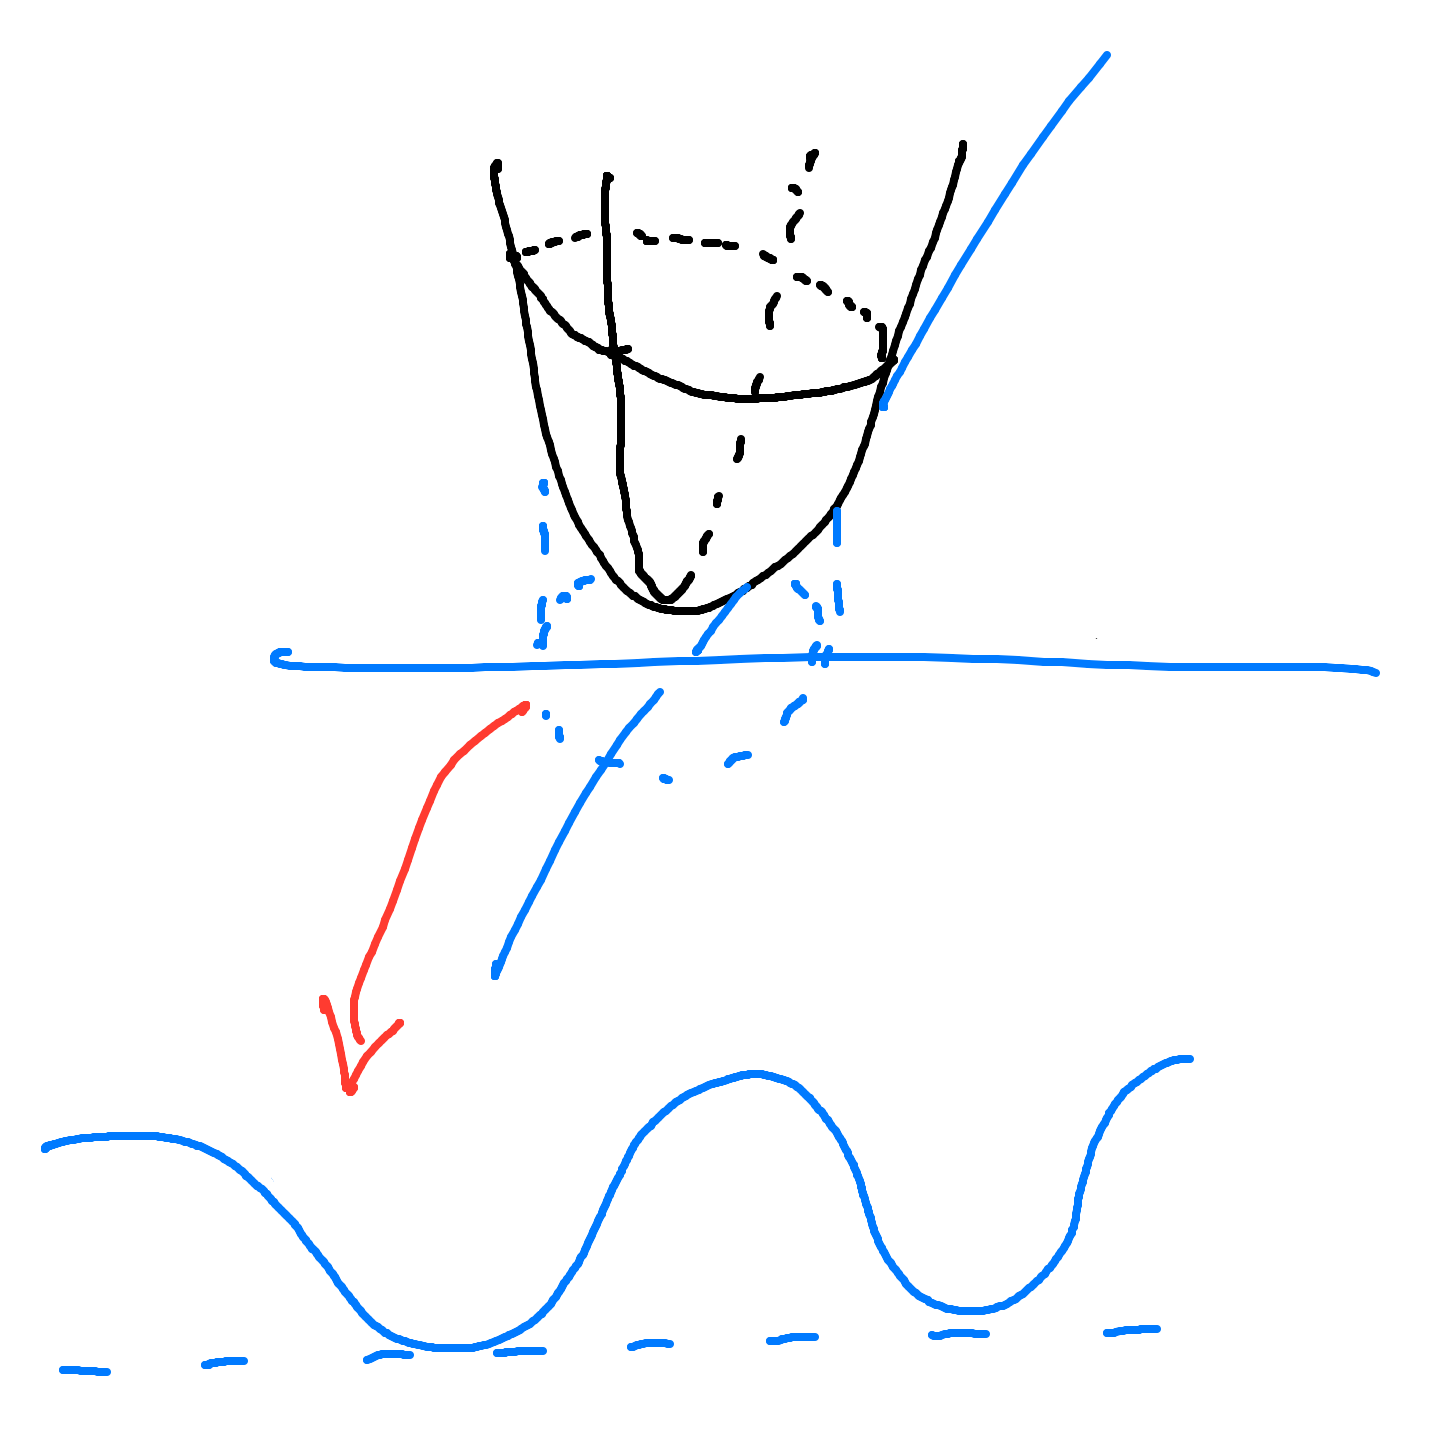
\includegraphics[width=10cm]{figs/PCA/Constrained-opt-eig.png}
\caption{Illustration of constrained optimization problem. The objective is a parabaloid constrained to the unit sphere. The parabaloid should look less symmetrical, but my drawing skills aren't great. Below, the unit sphere is unwrapped and the constrained objective is shown.}
\end{figure}

TODO: Connect this to the variational characterization of eigenvalues? 

Thus, if $n = 1$, we have found the subspace that provides maximal variance. For $n>1$, a similar technique can be used via an inductive argument. We won't follow the inductive argument through all the way here, but the idea is the following:

1. If you have an $r-1$ dimensional space of maximal variance, and you want to find the $r$, you subtract out the directions you've already found. (Draw a 2d picture for this.) Let
$$
\tilde X = X - \sum_{i=1}^{r-1} d_i d_i^\T X
$$
Here, we project $X$ onto each of the directions we've already found and subtract this from our dataset. (NOTE: Make sure $X$ contains $x_i$ as column vectors, otherwise need to use the transpose.) 
Let 
$$
\tilde S = \tilde X\tilde X^\T. 
$$
This is the sample covariance of the new data. Optimizing $\max_d^\T \tilde S d$ will give us the next direction of maximal variance. One may confirm that the eigenvalues of $\tilde S$ are the $d-r$th largest eigenvalues of $S$. (The larger eigenvalues, corresponding to directions we subtracted out are zero.) This is confirmed by expanding $\tilde X$ in the definition of $\tilde S$ and confirming that smaller eigenvalues of $S$ are eigenvalues of $\tilde S$. We see that the largest eigenvalues of $\tilde S$ gives us the next direction of maximal variance. 

TODO: What's missing from this proof is the inductive step. If we've found $d_{n-1}$, then how do I show that this really gives us the 2d subspace with optimal variance? 

\section{PCA: Minimum Reconstruction Loss Perspective}
TODO: Copy in other notes

\section{Interpreting PCA}
 In PCA, one can consider the latent codes or the projection to a lower dimensional subspace. The former can be thought of as a dimensionality reduction technique, while the latter may be thought of as a compression technique. 

To apply PCA, we choose some $r$ representing the number of principal components we wish to retain. Let $(v_i, \lambda_i)_{i=1}^r$ denote the $r$ largest eigenvalues/vectors, $v_i\in \R^d$. 
A data point, either from the training set, or a new point, is projected onto the principal components via
\begin{equation} \label{eq:PCA-proj}
\sum_{i=1}^r v_i v_i^\T z = \underbrace{(v_1,\ldots, v_r)}_{=: V} 
\begin{pmatrix}
v_1^\T\\
\vdots\\
v_r^\T
\end{pmatrix} z = \underbrace{V V^\T}_{=: P} z
\end{equation}
where $z\in \R^d$ is the point we wish to project. Note that $P: \R^d\to\R^d$. The projection $P$ takes data from $\R^d$ and embeds it onto a lower dimensional subspace in $\R^d$. The dimension of the subspace and the rank of $P$ are both $r$. This is illustrated in Figure \ref{fig:pca-proj}. 

\begin{figure}[h] \label{fig:pca-proj}
\centering
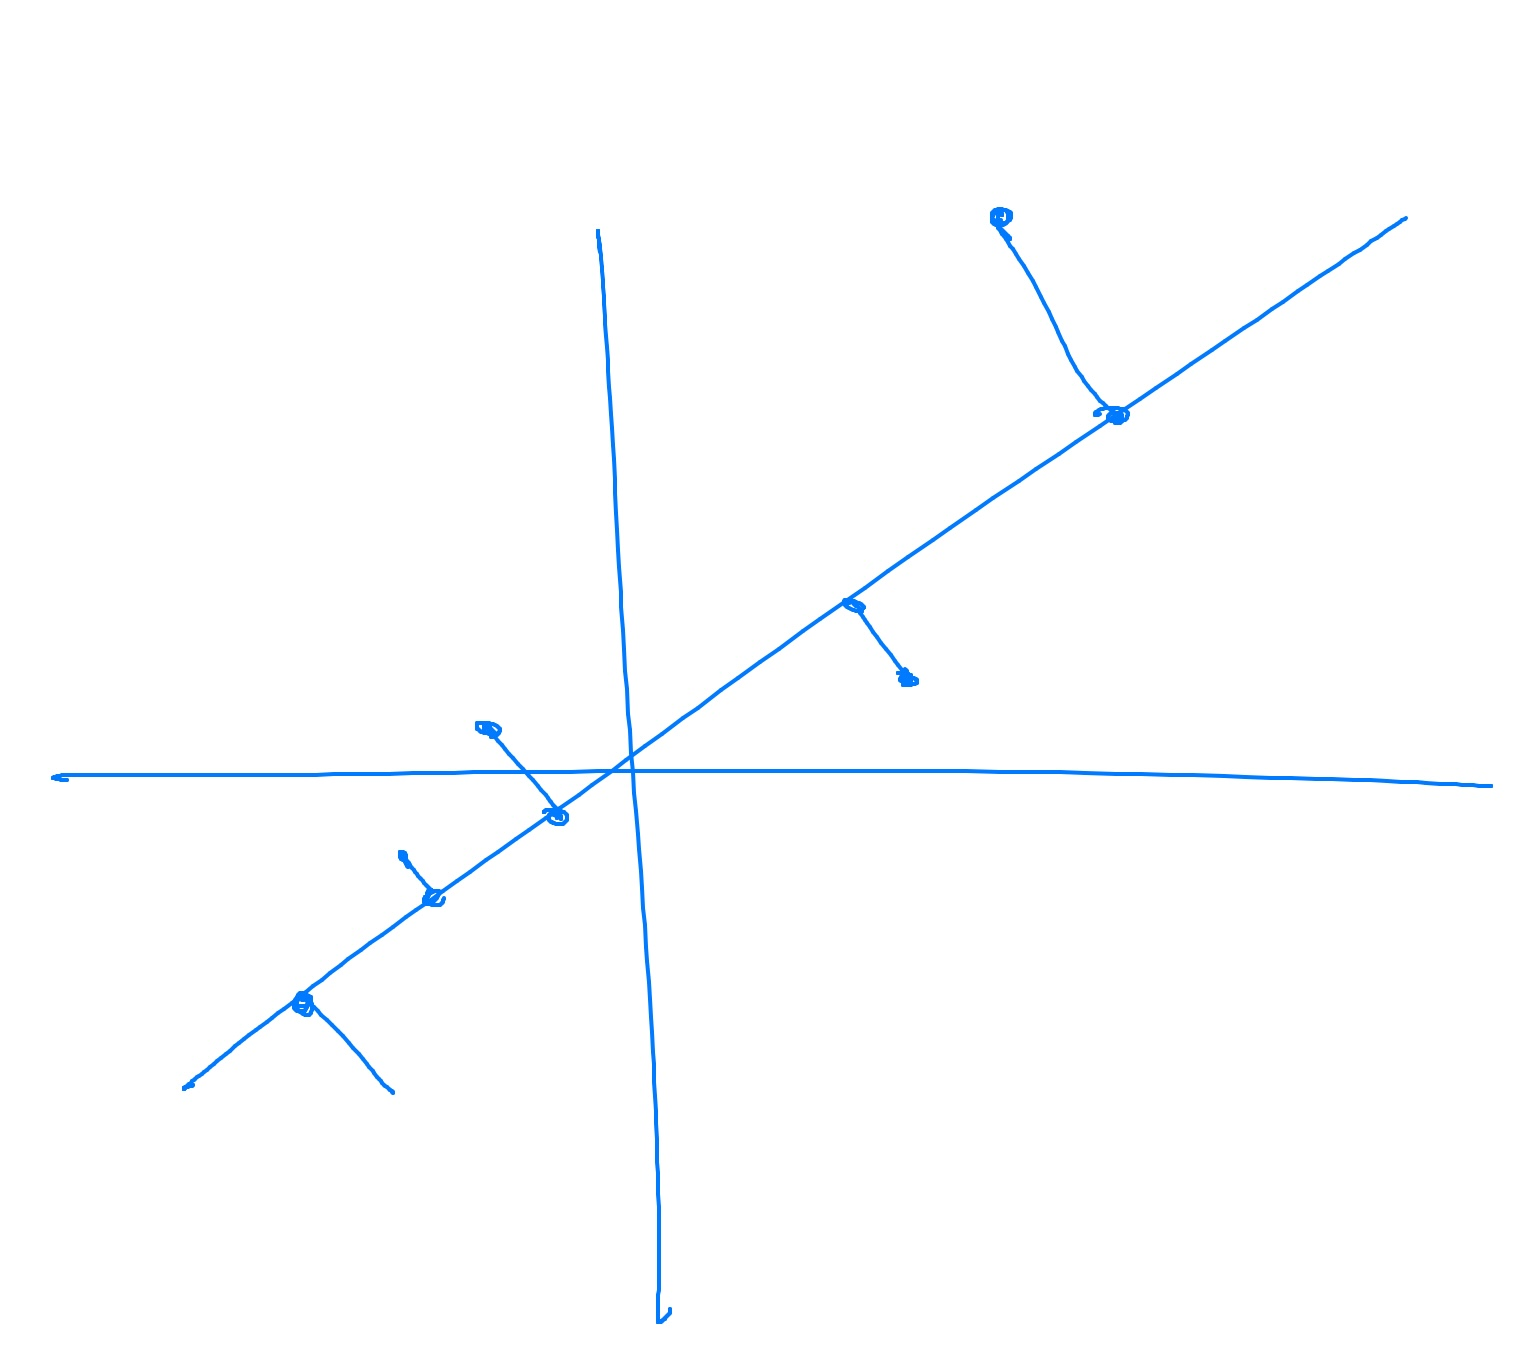
\includegraphics[width=8cm]{figs/PCA/PCA-proj.jpeg}
\caption{The projection operator $P$ embeds data to a lower dimensional subspace in $\R^d$}
\end{figure}

Note that in the sum in \eqref{eq:PCA-proj}, each eigenvector $v_i$ is multiplied by a coefficient $v_i^/T z$. We refer to these as the latent codes. In one to three dimensions, one may visualize these by treating them as coefficients of the canonical basis. This is illustrated in Figure \ref{fig:pca-latent-codes}. 
\begin{figure}[h] \label{fig:pca-latent-codes}
\centering
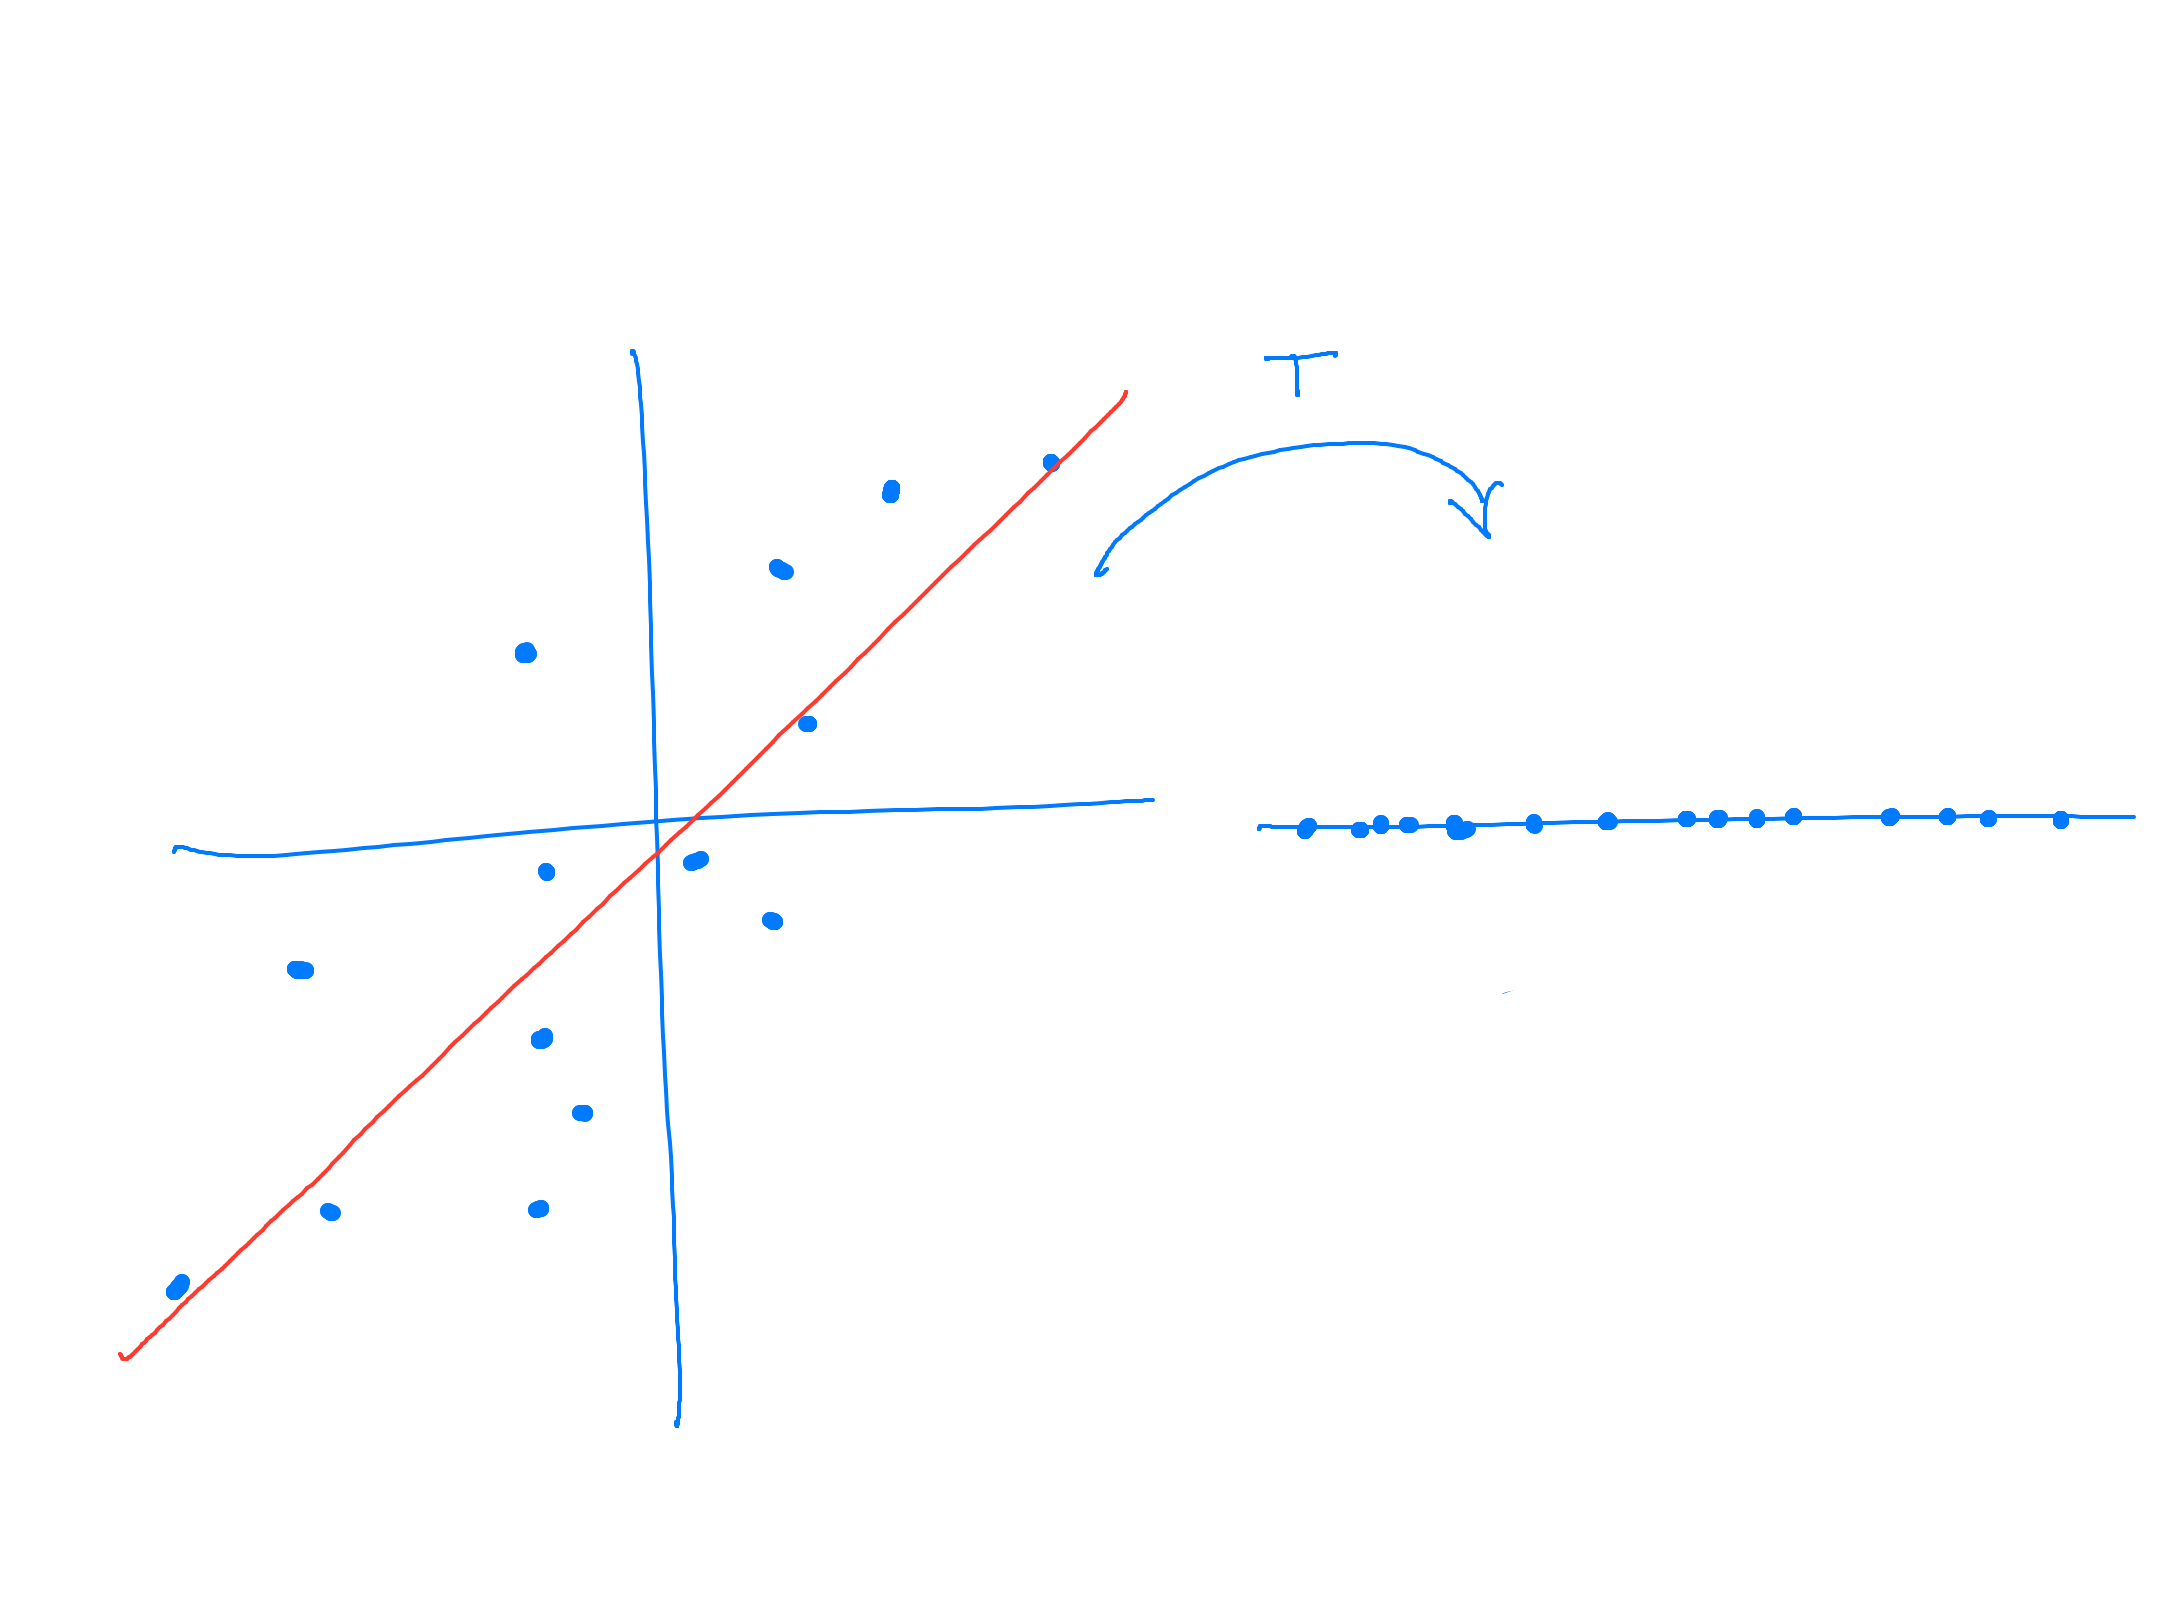
\includegraphics[width=10cm]{figs/PCA/PCA-latent-code.jpeg}
\caption{The projection operator $P$ embeds data to a lower dimensional subspace in $\R^d$.}
\end{figure}
Let
$$
T := 
\begin{pmatrix}
v_1^\T\\
\vdots\\
v_r^\T
\end{pmatrix}.
$$



\section{Examples}
TODO: Add Eigenfaces example. Note that this illustrates the "compression" aspect of PCA. Which is different from the dimensionality reduction. And it's kind of what the projection part is good for. 

\section{Unifying max variance and min reconstruction loss perspectives}
TODO: Ultimately, we're trying to optimize the same thing in both of these. Consider 2d example. One leg of a triangle is fixed between origin and data point. You have one degree of freedom to choose the other legs. You can maximize one leg, = maximizing variance. Or you can minimize another, which equates to minimizing reconstruction loss. See if this can be formalized a bit. 

\section{PCA and the Singular Value Decomposition}
IMPORTANT: In this section, I accidentally started using $X$ with $x_i$ as columns rather than rows. May not be consistent with rest of notes. Fix this. 

PCA reduces to computing the eigendecomposition of the sample covariance matrix $S = XX^\T$. In this section, we will see that this is equivalent to computing the SVD of $X$. 

\vspace{1em}
\noindent \textbf{SVD review:} For a possibly nonsquare matrix $A:\R^m\to\R^n$, the SVD involves computing a basis $(u_i)$ for the row and $(v_i)_i$ for the column space such that $Au_i = \sigma_i v_i$. Stick these basis vectors columnwise into matrics $U$ and $V$ so that $AU = V\Sigma $ or equivalently, $A = V\Sigma U^\T$, where $\Sigma$ has $(\sigma_i)$ on the diagonal. 
The singular values are computed by taking the eigendecomposition of $A^\T A$ and $A A^\T$. In particular, suppose that $(v_i)$ are an orthonormal set of eigenvectors of $AA^\T$ with eigenvalues $\sigma_i^2$ (exists by spectral theorem). Note that
$$
A A^\T v_i = \sigma_i^2 v_i \implies v_i^\T A A^\T v_i = \sigma_i^2 \|v_i\|^2 \implies \|Av_i\| = \sigma_i
$$
Let $u_i = \frac{1}{\sigma_i} A^\T v_i$, so that $u_i$ is unit norm. Note that
$$
AA^\T v_i = \sigma_i^2 v_i \iff A^\T A A^\T v_i = \sigma_i A v_i \iff A^\T A u_i = \sigma_i^2 u_i.
$$
Hence, $u_i$ is an eigenvector of $A^\T A$, and generally $(u_i)$ gives an orthonormal set of eigenvectors of $A^\T A$. 

\vspace{1em}
\noindent
\textbf{Back to PCA:} Returning to PCA, we see that computing the eigendecomposition of $XX^\T$ is equivalent to computing $V$ and $\Sigma$ in the SVD. 

In the SVD, one may retain only some of the singular vectors (is that what we call them) to obtain an optimal low-rank approximation to a matrix. This is summarized in the following result. 

\begin{theorem}[Ekhart-Mirsky-Young]
Let $A = V\Sigma U^\T$ and let $\Sigma_r = \myDiag(\sigma_1,\ldots, \sigma_r, 0,\ldots,0)$, where we use the convention that $\sigma_1\geq \sigma_2\geq \ldots$. Then $\hat A := V\Sigma_r U^\T$ is an optimal low rank approximation to $A$ in the senses that
$$
\|\hat A - A\|_F \leq \|B - A\|_F \mbox{ for all $B$ with rank $r$}
$$
and
$$
\|\hat A - A\|_2 \leq \|B - A\|_2 \mbox{ for all $B$ with rank $r$}.
$$
\end{theorem}
A note on proving this result: Proving the spectral norm component is easier. The Frobenius norm component requires (the approach I know of) using some tricks like Weyl's inequality. Both of these are nice exercises. 

\vspace{1em}
\textbf{Question}: How does this low-rank approximation perspective fit with PCA? 
The matrix of projected data points under PCA with $r$ principal components is given by 
$$
\tilde X = V_r V_r^\T X,
$$
where $V_r = (v_1,\ldots, v_r)$. On the other hand, the SVD low rank approximation of $X$ is given by
$$
\hat X = V \Sigma_r U^\T. 
$$
Note the former is simply a projection using the SVD basis vectors $V$ for the column space of $X$. The latter uses both basis vectors to map to singular value space, zero out unwanted components and then map back. Are these the same? 
To clarify this, let
$U_r\in \R^{d\times r}$ and $V_r \in \R^{m\times r}$, be matrices only retain the singular vectors corresponding to the $r$ largest singular values. Note that 
$$
\tilde X = V_r V_r^\T X = V_r V_r^\T V \Sigma U^\T = V_r [I_r, ~0] \Sigma U^\T = V_r \Sigma_r U_r^\T = V \Sigma_r U^\T = \hat X,
$$ 
where we have used the fact that V is constructed from an orthonormal basis. Hence, these are the same, and the projected data matrix $\tilde X$ in PCA is an optimal low-rank approximation to $X$. 
TODO: Clarify what each of these means. Double check the dimensions. Make sure everything works out. I don't want to be mapping from $\R^d$ to somewhere else, when mapping each column in $X$. 
Hence, despite the fact that PCA only computes $V$, it still allows us to construct an optimal low-rank approximation of $X$. 

\vspace{1em}
\noindent \textbf{High dimensional data}: An interesting follow on question from this is, what if $m \ll d$, i.e., data is very high-dimensional? If $d$ is large, then it may bay be expensive to compute the eigendecomposition of $S\in \R^{d\times d}$. But $U\in \R^{m\times m}$. Could we achieve the same results by computing $U$? The answer is yes, and follows readily from the SVD. Let $(u_i)$ be eigenvectors of $X^\T X\in \R^{m\times m}$. Note that this matrix doesn't have the same clean `covariance' interpretation (does it have a nice interpretation?). Let
$$
U_r = (u_1,\ldots, u_r)
$$
and let 
$$
\tilde X = XU_rU_r^\T.
$$
Applying the SVD to $X$ again, we see that this gives us the identical result to the standard PCA approach. It's interesting that here, the projection matrix is $\tilde X^\T = U_r U_r^\T X^\T$. We are now projecting rows of $X$ via the projection matrix $U_r U_r^\T$. Does this have a nice interpretation, like going to some nice subspace, like the minimum variance idea? 

\section{Kernel PCA}
In this section, we review Kernel PCA. I'm not exactly sure why people like Kernel PCA. 

TODO: Kernel PCA can follow as a really nice high-dimensional extension of PCA. But, I honestly don't get the point. I guess it's another way to visualize your data. But to what end? I haven't seen compelling examples visualizing, like, image datasets using kernel PCA. The most compelling example I can think of is that it's useful for better understanding kernel methods. Like, it lets you visualize a kernel method to some degree. What's I'm thinking is that I'm going to put a pin in this, and if I come back and study kernel methods, then I'll come back and flesh this section out. 

Plan: 
- The Bishop book as a clear exposition on deriving Kernel PCA that can basically be followed verbatim (I think... I actually only scanned that one)
- Two aspects of kernel PCA that intrigue me:
- Your data is mapped to a manifold. But when you project new data, you might actually not land on the manifold, so you can't go back to projected data. This idea seems interesting. 
- Examples with three concentric rings of data seem interesting. They can separate nicely with a linear separator. I'm still not entirely sure I understand the purpose of kernel PCA for this. Sure, it might help you to see clusters or something better. But nobody seems to know how to interpret it. 
- Honestly, if you really understood kernel PCA, could it be a powerful tool for really getting a good characterization of your data? Like, can you help people to interpret it better? Also, can you vary kernel parameters, like rbf bandwidth, to get a more complete characterization of your data topology?

%\section{Probabilistic PCA}
%
%\section{Autoencoders}
%
%\section{Variational Autoencoders}



\chapter{Other fun topics/one off topics}
\begin{itemize}
  \item Thompson sampling (just because)
  \item Gibbs sampling and other sampling techniques (let's be honest, this is it's own chapter)
\end{itemize}

\chapter{Other notes/Daily notes}
\section{Gaussian Distribution: Normalizing Constant 5/24/24}
The standard Gaussian distribution is given by $1/\sqrt{2\pi}\int e^{-\frac{1}{2}x^2/2}$. How do we know this is a valid density function? Specifically, how do we know the normalizing constant is 1? Here's a quick proof. 

Before starting, recall the change of variables formula
$$
\int_{G^{-1}(\Omega)} f(x)\dx = \int_\Omega f(G(x))|\det G(x)|dx.
$$
Here, $G$ is an invertible diffeomorphism. Now, what we're essentially looking for is to show that
$$
\int_-\infty^\infty \exp(-\frac{1}{2}x^2)\dx = \sqrt(2\pi). 
$$
The following trick allows us to compute it. Let $I = int_-\infty^\infty \exp(-\frac{1}{2}x^2)\dx$. We will compute $I^2$ instead of $I$. I'm not sure if there is some good intuition for why this is easier. But it works. We have
\begin{align}
I^2 & = \left( int_-\infty^\infty \exp(-\frac{1}{2}x^2)\dx \right)\left( int_-\infty^\infty \exp(-\frac{1}{2}x^2)\dx \right)\\
& = int_-\infty^\infty \exp(-\frac{1}{2}(x^2+ y^2))\dx.
\end{align}
This is amenable to a conversion to polar coordinates. Now, I'm sure we could apply the change of variables formula directly at this point. But with a little bit of cheating, I'm going to note that what I'd ultimately like to do is integrate over $r\geq 0$. I'm going to observe that if we consider polar coordinates, then integrating a ring of fixed radius from $\theta=0$ to $2\pi$, we have a density of $\int_0^{2\pi} e^{-r^2} d\theta = 2\pi r e^{-r^2}$. So, 
$$
I^2 = \int_{0}^\infty r e^{-\frac{1}{2}r^2}\dr.
$$
Now, apply change of variables. With $G(x) = \sqrt(2x)$ we see that
\begin{align}
I^2 & = 2\pi\int_{0}^\infty \sqrt{x} e^{-x} x^{-1/2} \dx\\
& = 2\pi \int_0^\infty e^{-x}\dx.
\end{align}
The last integral we know how to evaluate, and it evaluates to 1, so we see that $I^2 = 2\pi$ or $I = \sqrt{2\pi}$. 

\section{Polar Change of Coordinates}
When you do a polar change of coordinates, you change from $\dx \dy$ to $r\dr d\theta$. I get confused where the $r$ actually comes from. And, honestly, the way change of variables is applies is a little counterintuitive to me. So, I'm jotting it down. 
For completeness, recall the change of variables formula. 
$$
\int_{G^{-1}(\Omega)} f(x)\dx = \int_\Omega f(G(x))|\det DG(x)|dx.
$$
As a running example, we'll consider how to integrate $\int e^{-(x^2 + y^2)}$. To apply change of variables, let $f(G(r,\theta)) = e^{-r^2}$. The conversion from polar to cartesian is given by 
$$
G(r, \theta) = (r\cos \theta, ~r\sin \theta). 
$$
Let $H:= G^{-1}$ so that $f(x,y) = f(G(H(x, y)))$. Here, we have $H(x,y) = (x^2 + y^2, ~ \arctan{2}(y/x))$. So, we see that 
$$
f(x,y) = e^{x^2 + y^2}.
$$
In order to apply change of variables, note that 
$$
D_{(r,\theta)} G(r,\theta) = 
\begin{pmatrix}
\cos\theta & r\sin\theta\\
\sin\theta & r\cos\theta
\end{pmatrix},
$$
so that $|\det D G| = r(\sin^2\theta \cos^2\theta) = r$. Now, applying change of variables, we see that
$$
\int_{\R^2} e^{-(x^2 + y^2)} dL(\R^2) = \int_{\substack{r \geq 0\\ \theta \in [0, 2\pi)}} e^{-r^2} r dL(\R^2),
$$
where I'm trying to use that notation to denote the standard Lebesgue measure over $\R^2$. Note that if we let $\Omega$ be the domain on the right hand side, then $G^{-1}(\Omega)$ gives us the domain on the left hand side. I'm not sure if I'm actually doing that right, but this should be equivalent to
$$
\int_{\R^2} e^{-(x^2 + y^2)} \dx \dy = \int_{\substack{r \geq 0\\ \theta \in [0, 2\pi)}} e^{-r^2} r \dr d\theta.
$$
And, of course, in general, you have
$$
\int_{\R^2} f(x,y) \dx \dy = \int_{\substack{r \geq 0\\ \theta \in [0, 2\pi)}} f(G(r,\theta)) r \dr d\theta,
$$
where we've carefully defined what the functions on each side of that mean. 

\section{Change of Variables}
This section is about, in my opinion, one of the most useful and beautiful results in calculus. 
\begin{theorem}[Change of Variables] \label{thrm:CoV}
Suppose that $\Omega$ is an open subset of $\R^{n}$ and $G:\Omega\to \R^n$ is a $C^1$ diffeomorphism. If $f$ is $L^1$ integrable over $G(\Omega)$, then 
\begin{equation} \label{eq:CoV}
\int_{G(\Omega)} f(x) \dx = \int_{\Omega} f(G(x)) \,\left| \det DG(x) \right| \dx.
\end{equation}
\end{theorem}
Above, $DG(x)$ is the Jacobian determinant of $G$. 

Sometimes, when integrating, it is helpful to do a change of variables in order to massage an integral into a form that is easier to handle. This change of variables is represented by $G(x)$ inside the integral. However, simply modifying the argument to the integral changes the value of the integral. The change of variables formula tells us the necessary correction term inside the integral. This is $\left| \det DG(x)\right| $. We'll build intuition for what this correction term means later on. But first, we'll go over a few examples to illustrate how eminently useful this result is. 

\vspace{1em}
\noindent 
\textbf{Example:} Change of variables is the multivariable generalization of $u$ substitution, familiar from introductory calculus. Anytime you use $u$-substitution to reformulate some tricky integral, you're using the change of variables formula.  

\vspace{1em} \noindent 
\textbf{Example (Function of a RV)}: Suppose that $X \in \R^n$ is a random variable with density function $f_X$. Let $Y\in \R^n$, with $Y = g(X)$ where $g$ is a $C^1$ diffeomorphism. What is the density function of $Y$? This is an important question that arises often in ML applications and elsewhere. Ignoring questions of measurability, note that for a set $A\subset R^n$ 
\begin{align}
\P(Y \in A) = \P(g(X) \in A) = \P(X \in g^{-1}(A)) = \int_{g^{-1}(A)} f_X(x)\dx. 
\end{align}
Let $h =g^{-1}$ to make notation clearer. Applying change of variables we see that
$$
\int_{h(A)} f_X(x)\dx = \int_A f_X(h(y)) |\det Dh(y))\dy. 
$$
where in the second line we somewhat arbitrarily change the variable of integration from $x$ to $y$ to make the connection to the density $f_Y$ clearer.
Hence,
$$
\P(Y\in A) = \int_A f_X(h(y)) |\det Dh(y))|\dy
$$
Since this holds for all $A$ (ignoring measurability considerations), we see that the integrand on the RHS must be the density of $Y$, hence
\begin{equation} \label{eq:pushforwardY} % is this the pushforward?? TODO: Double check. 
f_Y(y) = f_X(h(y)) |\det Dh(y))|.
\end{equation}
Any time you need an analytic expression for a function of a random variable, the change of variables formula is indispensable. 

For a concrete example of this, suppose that $X$ is uniformly distributed on $[0,1]$ and $Y = X^2$. What is the density of $Y$? It's $f_Y(y) = \frac{1}{2}\frac{1}{\sqrt{y}}$. This is shown in Figure \ref{fig:cov-example1}. Also, see demo in Jupyter notebook.
\begin{figure}[h] \label{fig:cov-example1}
\centering
\centering
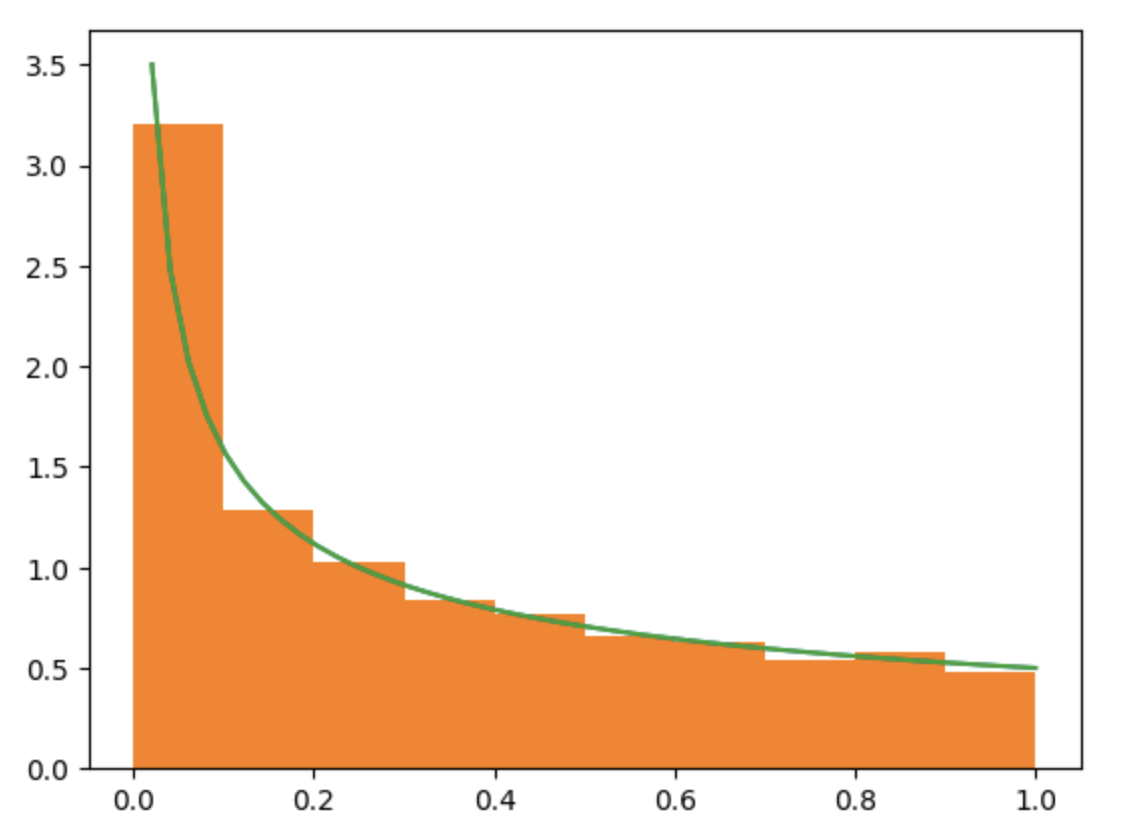
\includegraphics[scale = .5]{change_of_variables/cov-example1.png}
\caption{Density of $Y = X^2$, $X\sim U([0,1])$}
\end{figure}

\vspace{1em} \noindent 
\textbf{Example (Normalizing Flow)}: Suppose we have a set of points $(z_i)_i $ where each $z_i \sim p$, i.i.d, where $p$ is some density function. Suppose that we would like to model the density $p$. Consider a change of variables-based approach. Let $f$ be some distribution we know how to sample from easily (e.g., normal or uniform density). Suppose we sample $W\sim f$ and then pass it through some parametric function $g_\theta(x)$, which we assume to be a $C^1$ diffeomorphism. We wish the random variable $Z=g_\theta(W)$ to have a density as similar as $p$ as possible. Letting $h_\theta = g_\theta^{-1}$, change of variables tells us that the density function of $Z=g_\theta(W)$ is
\begin{equation} \label{eq:NF-density}
f(z;\theta) = f(h_\theta(z)) |\det D_z h_\theta(z)| 
\end{equation}
We may fit $f(z; \theta)$ to our dataset $(z_i)$ using a maximum likelihood approach. If we assume $(z_i)$ is iid, then the likelihood of the joint sample is
\begin{equation} 
L(\theta) = \prod_i f(z_i; \theta)  = \prod_i f(h_\theta(z_i)) |\det D_z h_\theta(z_i)|,
\end{equation}
and the negative log likelihood is
\begin{equation} \label{eq:NF-objective}
\ell(\theta) = -\sum_i \left[ \log f(h_\theta(z_i))  + \log |\det D_z h_\theta(z_i)| \right].
\end{equation}
Minimizing \eqref{eq:NF-objective} simply maximizes the likelihood of the data under our model. This provides us with a function $h_\theta$ that allows us to draw samples from an approximation to $p$. Once $\ell$ is minimized, if we let $Z = h^{-1}_\theta(X)$ for $X\sim f$, then the density of $Z$ is approximately $p$. Methods exist for obtaining $h^{-1}_\theta$. Also, if we simply wish to evaluate the approximate density of $p$ at test point, then we simply use \eqref{eq:NF-density}. This method of approximating a density is called a normalizing flow, and is a current research area in ML. There is \emph{a lot} we could say about this, but we'll ignore it to stay focused on CoV for now. Maybe save this for another time.

\vspace{1em} \noindent
\textbf{Example (Law of the unconscious statistician)}: Let $X$ be a random variable with density function $f_X$. Let $g$ be some measurable function. What is the expected value of $g(X)$? It is commonly taken to be, by definition,
\begin{equation} \label{eq:LOTUS}
\E[g(X)] = \int g(X) f_X(x)\dx. 
\end{equation}
\emph{However}, this is not obvious. This is so commonly taken to be the definition of $\E[g(X)]$ that it is known as the law of the unconscious statistician. 

The definition of the expectation of a random variable is
$$
\E[Z] := \int x f_Z(z) dz. 
$$
Consider the simple case where $X$ is scalar-valued and $g$ is a $C^1$ diffeomorphism. Applying \eqref{eq:pushforwardY}, we know that the density function for $Y = g(X)$ is
$$
f_Y(y) = f_X(g^{-1}(y)) |(g^{-1}(y)')
$$
and 
$$
\E[g(X)] = \int y f_X(g^{-1}(y)) |(g^{-1}(y)') \dy. 
$$
Now, apply change of variables again with $y = g(x)$. To do this, we just substitute $g(x)$ in for $y$ above and multiply by $g'(x)$ inside the integral. We arrive at
\begin{align}
\E[g(X)] & = \int g(x) f_X(x) \frac{d}{dy} g^{-1}(\underbrace{g(x)}_{=y}) g'(x) \dx\\
& = \int g(x) f_X(x) \dx,
\end{align}
where in the last line, we recognize from the chain rule that $\frac{d}{dy} g^{-1}(g(x)) g'(x)  = \frac{d}{dx} g^{-1}(g(x)) = 1$. 
Hence, \eqref{eq:LOTUS} is correct. But the result isn't obvious. Here, we only showed it in a simple scalar-valued case with invertible and differentiable $g$. It does hold more broadly. A measure-theoretic treatment shows that it holds when $g$ is a measurable function and the random variable $X$ has a finite mean (I think... double check). 

\vspace{1em} \noindent
\textbf{Example (Reparameterization Trick)}: The CoV formula is critical in using the reparameterization trick, which is the foundation of an important class of variational-inference based methods in ML. Save the details for another time, for the sake of brevity. 

\vspace{1em}
\noindent
\textbf{Example (Polar change of coordinates/Gaussian normalization constant)}: 
Consider evaluating the integral 
\begin{equation}\label{eq:gauss-soln-step}
I = \int e^{-\frac{1}{2}(x^2 + y^2)} \dx \dy. 
\end{equation}
TODO: Just added in the 1/2 above. Make consistent through the rest! It should already be consistent after the easter egg. 
(We'll see at the end why this is actually an extremely useful integral to know.) This integral is radially symmetric and will be easier to evaluate in polar coordinates, where $x = r\cos\theta$ and $y=r\sin\theta$. 
%The application of change of variables here is a bit subtle. (Basically, it's easier to go from polar to cartesian, so we force ourselves to work primarily in that direction.) 
%Let $f$ be the integrand above, and let $G$ be a function such that $f(G(r,\theta)) = e^{-r^2}$. 
The conversion from polar to cartesian is given by the function
$$
G(r, \theta) = (r\cos \theta, ~r\sin \theta). 
$$
Letting $f(x,y)$ be the integrand above, we have
$$
f(G(r,\theta)) = \exp( -(r^2\cos^2\theta + r^2 \sin^2 \theta)) = \exp(-r^2).
$$
%Let $H:= G^{-1}$ so that $f(x,y) = f(G(H(x, y)))$. Here, we have $H(x,y) = (x^2 + y^2, ~ \arctan{2}(y/x))$. So, we see that 
%$$
%f(x,y) = e^{x^2 + y^2}.
%$$
In order to apply change of variables, note that 
$$
D_{(r,\theta)} G(r,\theta) = 
\begin{pmatrix}
\cos\theta & -r\sin\theta\\
\sin\theta & r\cos\theta
\end{pmatrix},
$$
so that $|\det D G| = r(\sin^2\theta \cos^2\theta) = r$. Now, applying change of variables, we see that
$$
\int_{\R^2} e^{-(x^2 + y^2)} dL(\R^2) = \int_{\substack{r \geq 0\\ \theta \in [0, 2\pi)}} e^{-r^2} r dL(\R^2),
$$
where I'm trying to use that notation to denote the standard Lebesgue measure over $\R^2$. Note that if we let $\Omega$ be the domain on the right hand side, then $G^{-1}(\Omega)$ gives us the domain on the left hand side. I'm not sure if I'm actually doing that right, but this should be equivalent to
$$
\int_{\R^2} e^{-(x^2 + y^2)} \dx \dy = \int_{\substack{r \geq 0\\ \theta \in [0, 2\pi)}} e^{-r^2} r \dr d\theta.
$$
And, of course, in general, you have
$$
\int_{\R^2} f(x,y) \dx \dy = \int_{\substack{r \geq 0\\ \theta \in [0, 2\pi)}} f(G(r,\theta)) r \dr d\theta,
$$
where we've carefully defined what the functions on each side of that mean. 

As a final easter egg in this example, note that 
\begin{align}
I = \int_{\substack{r \geq 0\\ \theta \in [0, 2\pi)}} e^{-\frac{1}{2}r^2} r \dr d\theta = 2\pi \int \exp(-r^2) r\dr. 
\end{align}
Applying another change of variables where we let $r = G(u) = u^{1/2}$ we get (I might have missed a minus sign below...)
$$
I = 2\pi \int_0^\infty \exp(-\frac{1}{2}u) du = 2\pi. 
$$
So, we have an explicit evaluation of this integral. But, note that
$$
\left(\int \exp(-\frac{1}{2}x^2) \dx\right)^2 = I
$$
You can see this by just expanding the square explicitly, and then combining everything under a double integral to get \eqref{eq:gauss-soln-step}. So, 
$$
\int \exp(-\frac{1}{2}x^2)\dx = \sqrt{2\pi}. 
$$
or, equivalently, 
$$
\frac{1}{\sqrt{2\pi}}\int \exp(-\frac{1}{2}x^2)\dx = 1
$$
This is how we know what the normalizing constant is for a normal random variable. 
End example. 

\vspace{1em}
\noindent
\textbf{Example} A high-dimensional gaussian is concentrated on the surface of a sphere. Change of variables is useful in deriving this. (Will do later.) 

\vspace{1em}
\noindent
\textbf{Bonus Example 1}: How can you sample from the unit 2sphere (embedded in $R^3$)? Consider using polar coordinates, so $\theta\in [0, 2\pi]$ is an azimuth and $\phi\in [0, \pi]$ is an elevation (This is an angle measured from the north pole.) Can you just sample $\theta, \phi$ uniformly from their sets? (Pause and consider.) Answer: No. To see why, consider a change of variables from uniform to polar coordinates. Suppose that $A$ is some subset of the unit sphere. Then under a uniform distribution on the unit sphere, we have
$$
\P(A) = \frac{1}{4\pi}\int_{A} 1\dx\dy\dz = \frac{1}{4\pi}\int_{g^{-1}(A)} \sin(\phi) \,d\phi \,d\theta,
$$
where we have used the fact that the surface are of the unit sphere is $4\pi$ and the fact that the spherical change of coordinates (see Figure \ref{fig:spherical-coords}) so that
\begin{align}
x = r\sin(\phi)\cos(\theta) \\
y = r\sin(\phi)\sin(\theta) \\
z = r\cos(\phi). 
\end{align}
\begin{figure}[h]

     \centering
     \begin{subfigure}[b]{0.4\textwidth}
         \centering
         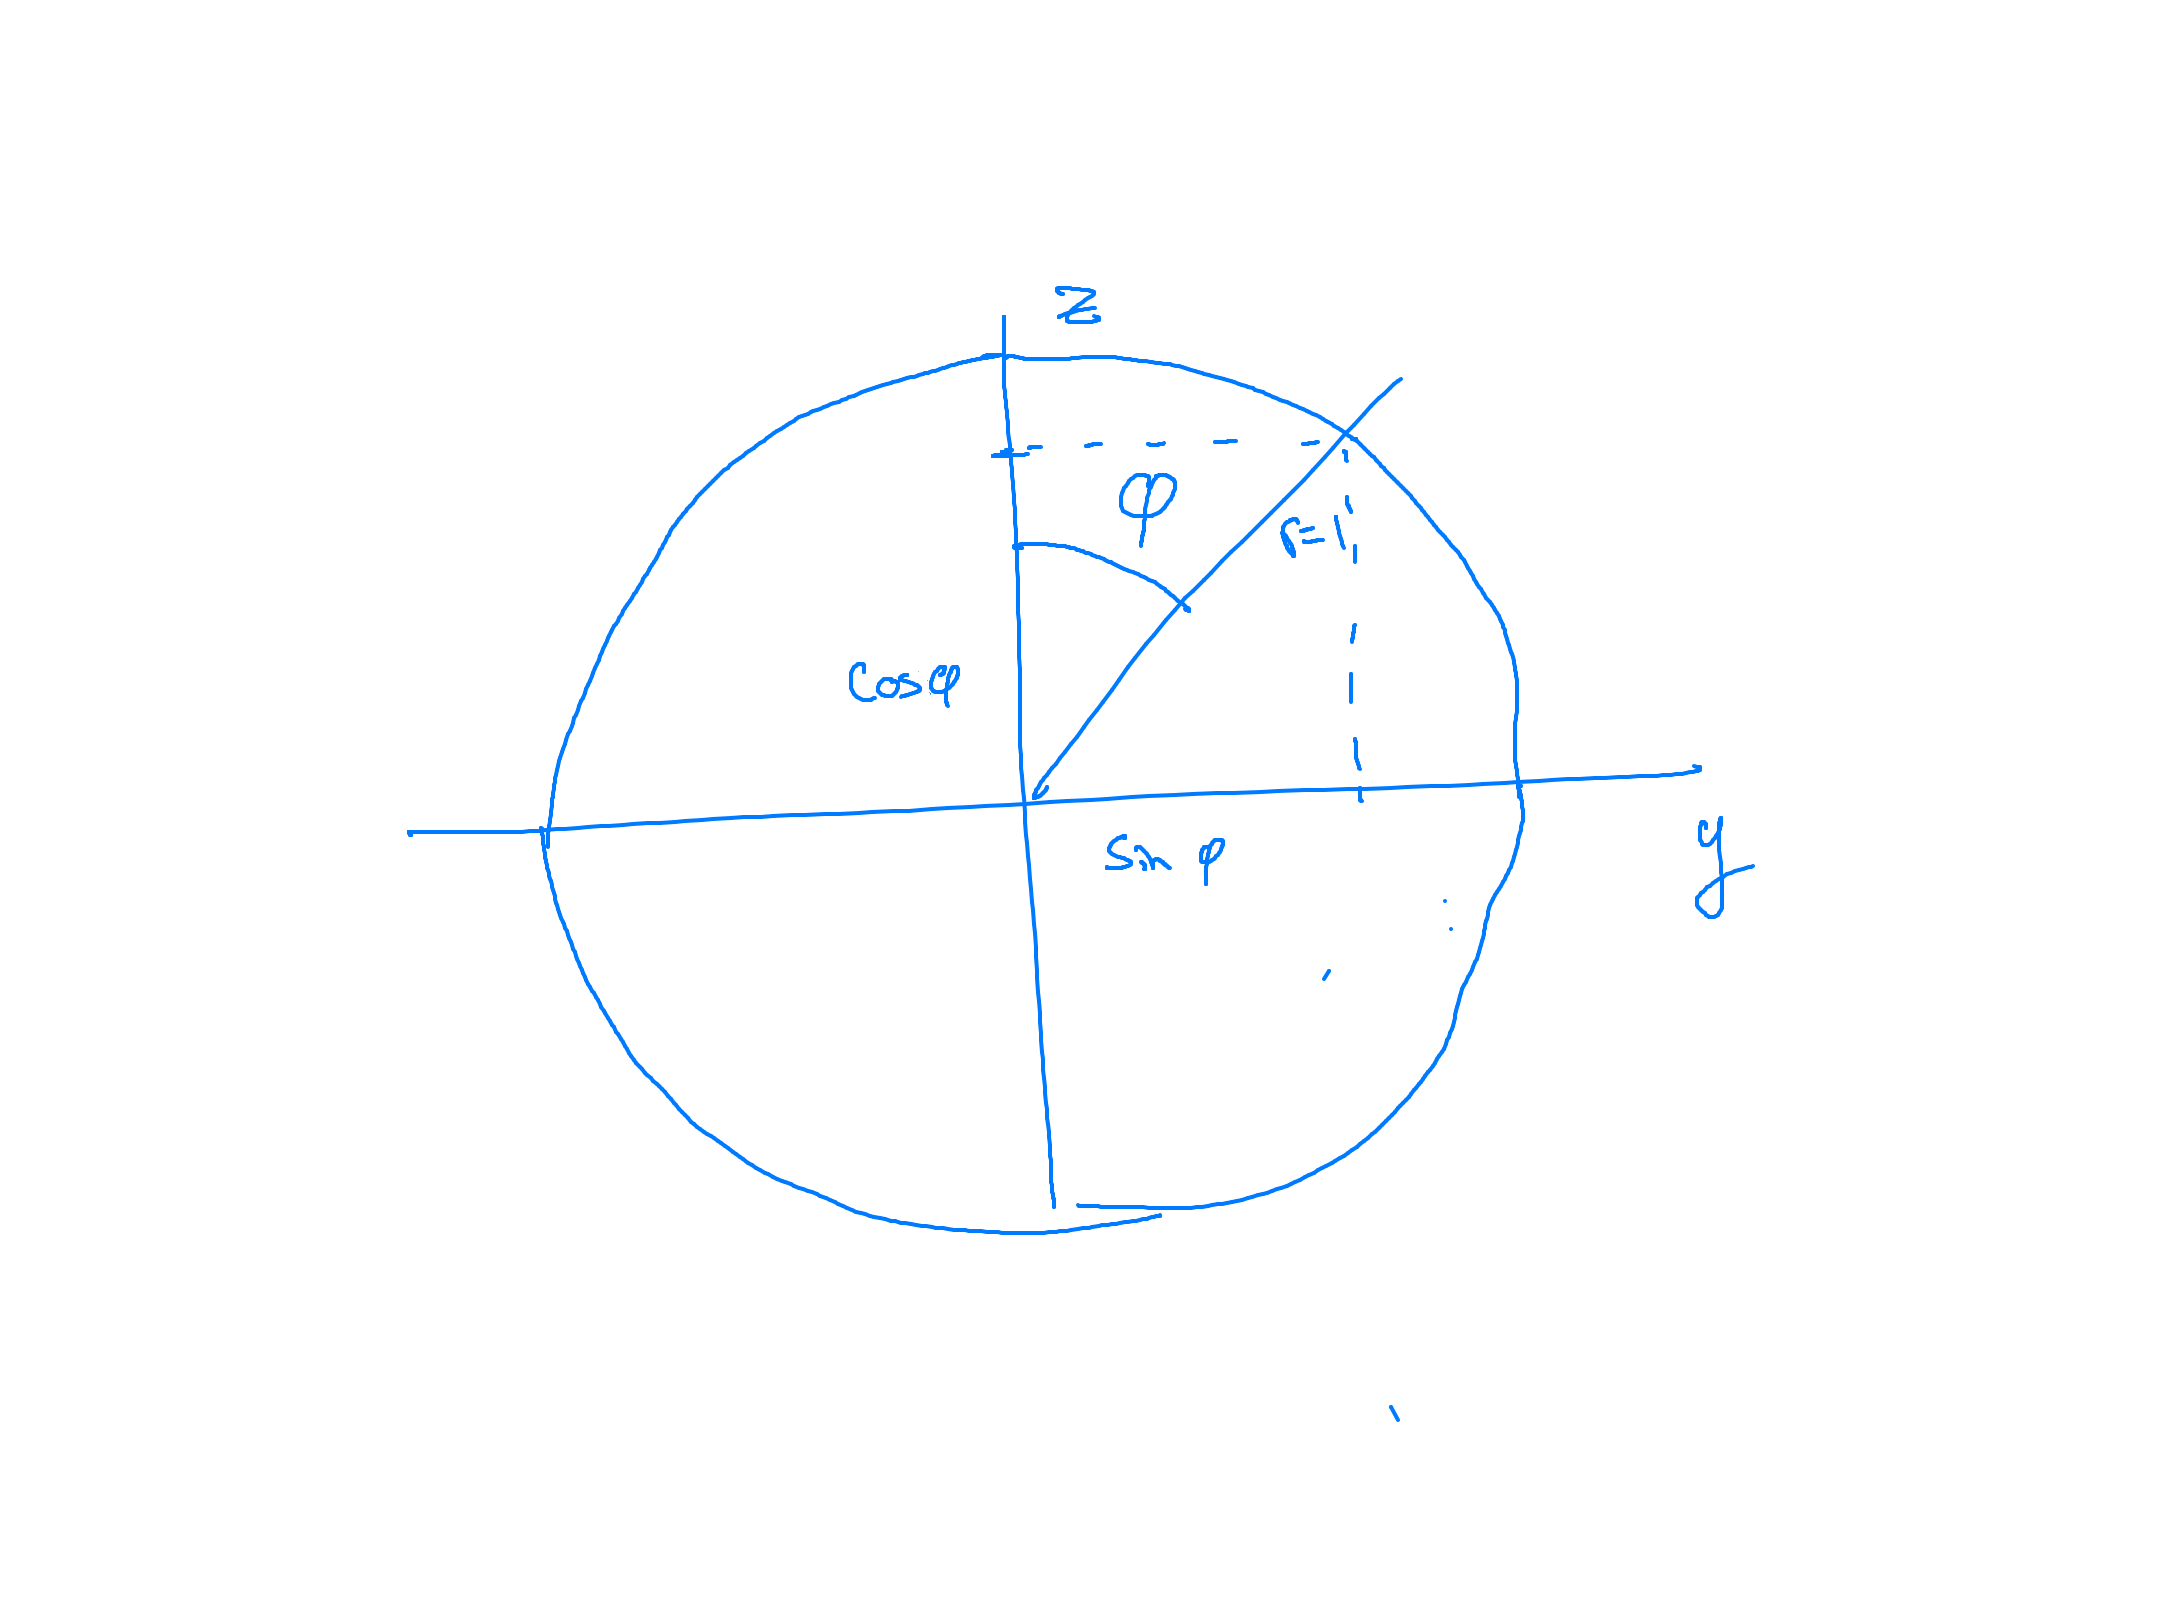
\includegraphics[width=\textwidth]{change_of_variables/spherical-coords1.jpeg}
         \caption{}
     \end{subfigure}
     \begin{subfigure}[b]{0.4\textwidth}
         \centering
         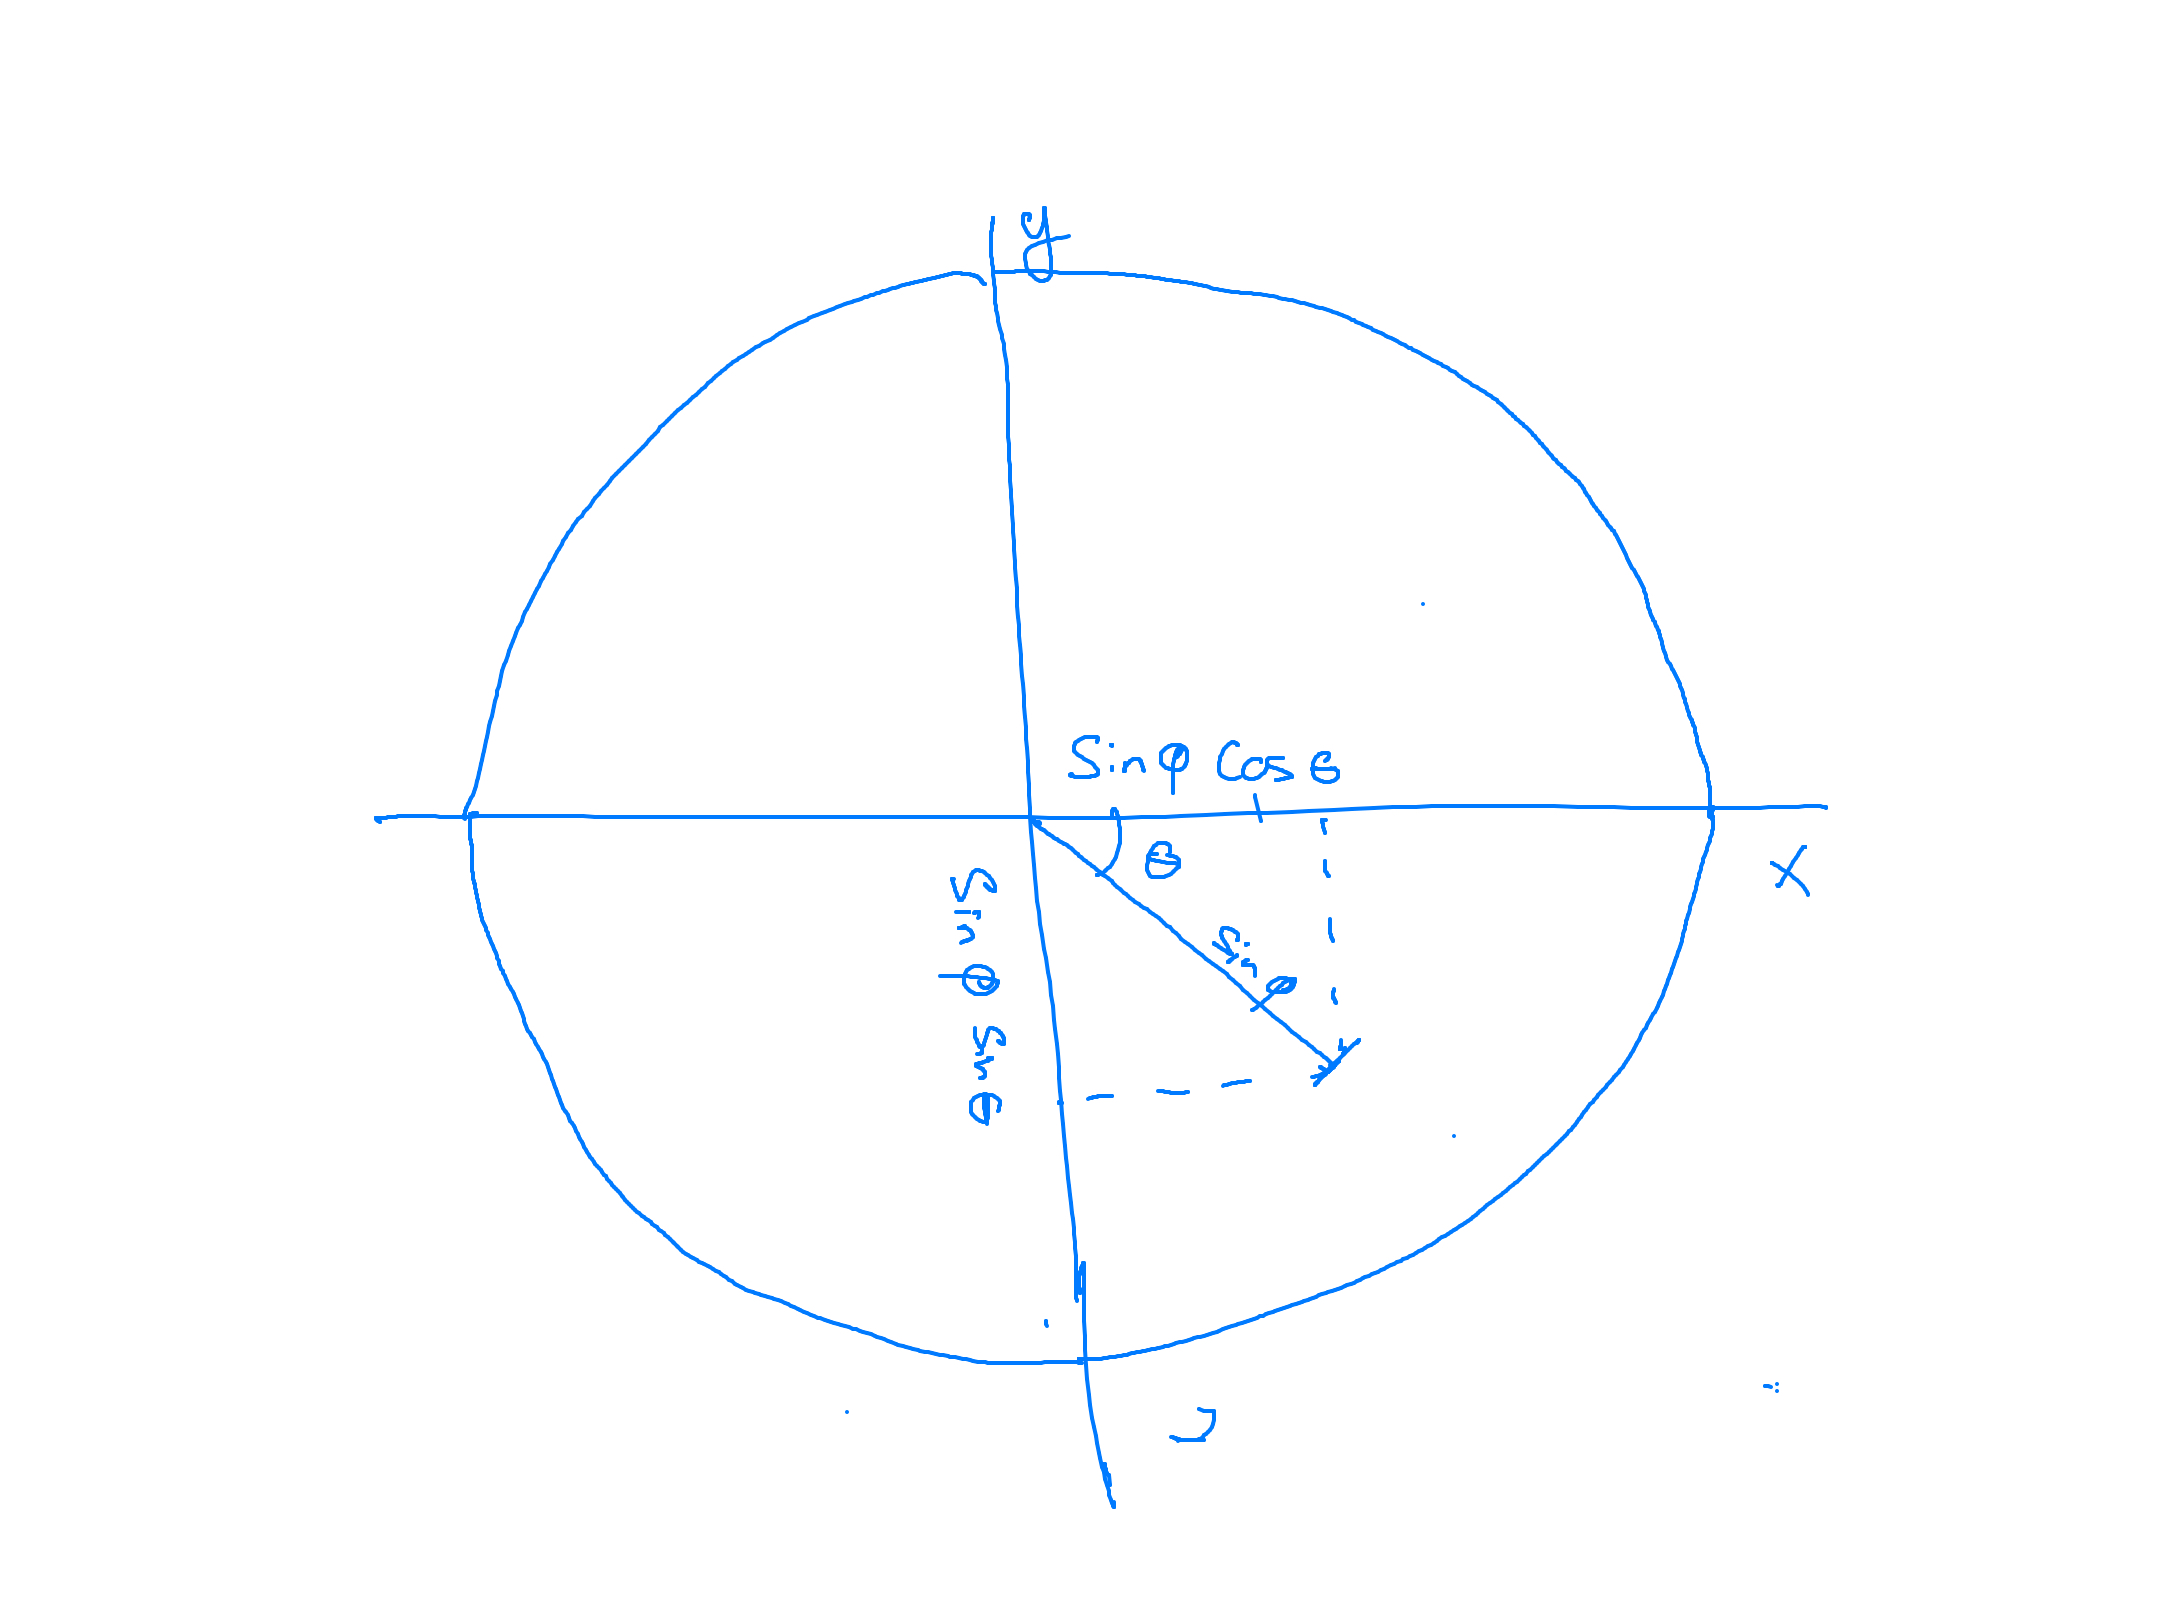
\includegraphics[width=\textwidth]{change_of_variables/spherical-coords2.jpeg}
         \caption{}
         \label{fig:three sin x}
     \end{subfigure}
        \caption{Spherical coordinates. I accidentally left out the $r$ in this figure. So just multiply everything by a radius $r$.}
        \label{fig:spherical-coords}
\end{figure}
The $\sin(\phi)$ comes from computing $\det DJ(\theta, \phi, r) = r^2\sin(\theta)$.\footnote{This actually raises an important subtlety. If we don't fix $r=1$, then we are going from $\R^3\to \R^3$. The Jacobian is invertible. If we do fix $r=1$, then we have 3 cartesian coordinates and 2 polar coordinates. And change of variables can't be applied. We get around this by computing the change of variables for 3 to 3 coordinates, and then fixing $r=1$, and then integrating only with respect to the two dimensional Lebesgue measure w.r.t. the angles. But this feels like it's playing a bit fast and loose.}
The integrand on the right hand side gives us the density for $\phi, \theta$ that corresponds to a uniform distribution on the sphere. In particular, the density to sample uniformly from the unit sphere in spherical coordinates is
$$
f(\theta, \phi) = \frac{1}{4\pi}\sin(\phi)\ones_{[0, 2\pi]\times [0, \pi]}.
$$
How do you sample from this distribution? Here's a trick that works, that I haven't thought through how you'd come up with from scratch. Let $u,v\sim U([0,1]^2)$. Let $\theta = 2\pi u$ and $v = \cos^{-1}(2v-1)$. Letting
$$
h(\theta, \phi) = g^{-1}(\theta, \phi) = 
\begin{pmatrix}
1/2\pi \theta\\
(\cos(\phi) - 1)/2
\end{pmatrix}
$$ and 
applying \eqref{eq:pushforwardY} we immediately get that $f_{\theta, \phi}(\theta, \phi) = \frac{1}{4\pi}\sin(\phi)$. The domain of the density comes from looking at the range $g(u, v)$. 

It should be noted that this is the hard way of sampling from the unit sphere. The easy way is to sample from a gaussian and then normalizing the samples. But this examples builds intuition that I think can generally be helpful. 

\textbf{Bonus Example 2}: 
Suppose you want to uniformly sample from the set of all rotation matrices in three dimensions. How can you do that? A rotation consists of an axis of rotation and an angle of rotation. You can uniformly pick the axis of rotation as above, and then sample an angle of rotation uniformly from $[0, 2\pi]$. Question: How do you sample a random rotation matrix in higher dimensions? Not sure...


\vspace{1em}
\subsubsection{Building Intuition}

The previous examples have demonstrated the clear utility of being able to change variables inside of an integral. The key term in CoV is the correction term $\left| \det DG(x) \right| $. This gives us the exchange rate required to compensate for the introduction of $g(x)$ inside the integrand. To build intuition about this, consider the example $f(x) = \frac{1}{2}x^2$. Suppose, for some made up reason, that we wish to evaluate the integral $\int_{[0,1]} f(x)\dx$, but we only have access to $f(g(x))$, where $g(x) = cx$, $c>1$.\footnote{We keep $c>0$ to make the discussion of ``compression'' consistent later. But the same reasoning holds for any $c\not=0$, just change the terminology to ``dilation'' where necessary.}
%First, note that 
%$$
%\int_{[0,1]} \frac{1}{2} x^2 = 1. 
%$$
%Now, suppose it is easier for some reason to evaluate the integral by substituting in $y = cx$. We wish to evaluate this same integral, but under the change of variables. 
\begin{figure}[h] \label{fig:cov-compression}
\centering
\centering
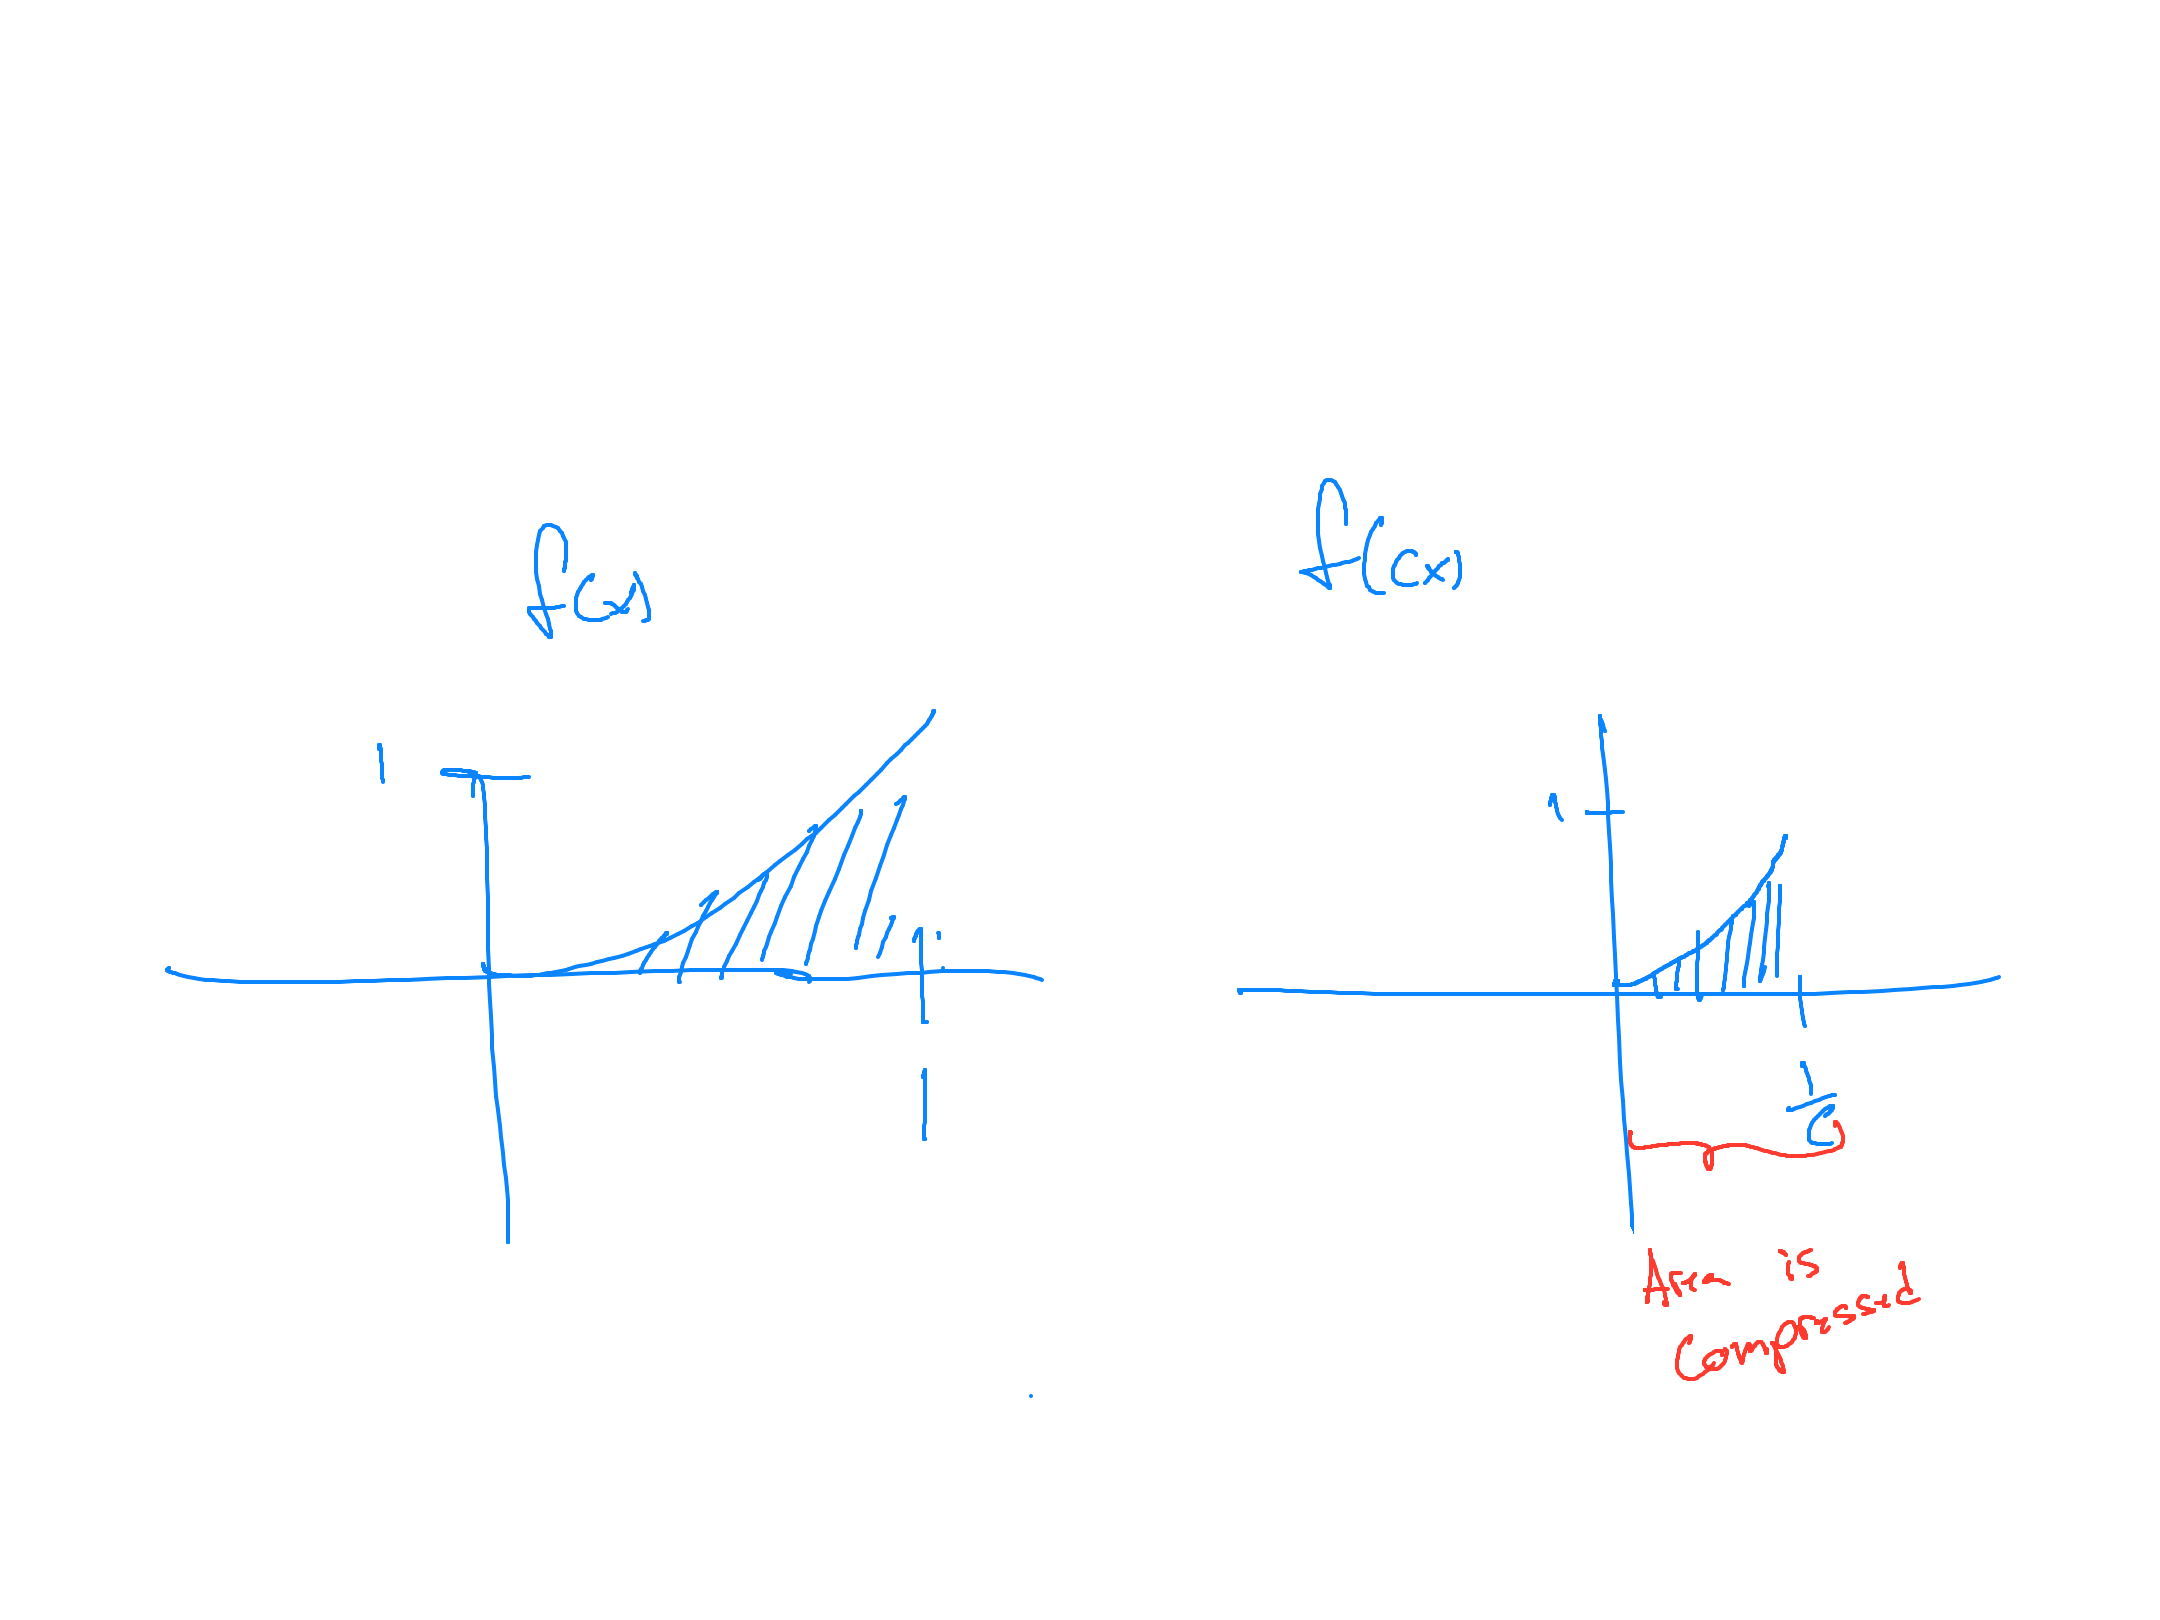
\includegraphics[scale = .21]{change_of_variables/CoV-compression.jpeg}
\caption{Illustration of ''compression'' effect.}
\end{figure}
The first thing to notice is that if we're going to evaluate the same integral, we've got to make sure the underlying domains match up. This is illustrated in Figure \ref{fig:cov-compression}. The function $g(x) = cx$ has the effect of compressing the domain of integration. The end point for integration inside the function is reached when $x=1/c$.  We make sure the domains match up by taking the preimage of the desired domain under $g$. Equivalently, we may state this as they do in Theorem \ref{thrm:CoV} in terms of $g$ rather than the primage, via 
$$
\int_{g(\Omega)} f(x)\dx = \int_{\Omega} \mbox{stuff}.
$$
Next, because $g$ compresses the domain of integration, if we directly integrate, we will end up with a value that is too small. Again, see Figure \ref{fig:cov-compression}. We compensate for this compression term by understanding the ``compression rate'' and compensating for it when computing the integral. I'm going to call this the exchange rate. The ``exchange rate'' at which it compresses can be understood by looking at the preimage of the canonical volume-1 set $[0,1]$. This tells us the volume of the set that maps to $[0,1]$. The exchange rate is given by the ratio. 
$$
\frac{\mbox{vol}\, [0,1]}{\mbox{vol} \, g^{-1}([0, 1])}.
$$
Evaluating this expression we get a ``compression ratio'' (I'm making that term up) of $c$. Higher compression ratio means more compressive. 
Because the function $g$ is linear, we can also get the exchange rate by just looking at the ratio
$$
\frac{\mbox{vol} \, g([0, 1])}{\mbox{vol}\, [0,1]}.
$$
This tells us the relative size of the set that $[0,1]$ is mapped to, and gives us the same information about the compression rate in the previous expression. Evaluating this expression gives us the same compression ratio. This ratio tells us the effect that including $g$ inside the argument of $f$ has. In particular, it tells us the rate at which infinitessimal segments are compressed inside the integral. We may now compensate for the infinitetessimal compression effect inside the integral by multiplying by the exchange rate
$$
\int_{[0,1]} \frac{1}{2} x^2 \dx = \int_{[0,1/c]} \frac{1}{2} (cx)^2  c\dx = 1
$$
%Note that in the a nonlinear case, we'd have to be careful to multiply by the local exchange rate--here, linearity gives us a global exchange rate. 
%Returning to linear maps, 
This same idea holds more generally if we consider the effect of a bijective linear map $T:\R^n\to\R^n$. The following result is critical. 
\begin{theorem}
Let $T:\R^n\to\R^n$. Then the image of the hypercube $T([0, 1]^n)$ is a parallelipiped. Representing $T$ as a matrix, the (signed) volume of the parallelipiped is given by $\det T$. 
\end{theorem}
In the previous theorem, the sign on the volume tells us about the orientation of the parallelipiped relative to the original hypercube. We won't go into that here. Taking $|\det T|$ gives the unsigned volume. 

\vspace{1em}
Example: Consider the matrix
$$
T = 
\begin{pmatrix}
0 & 1\\
2 & 3
\end{pmatrix}. 
$$
The image of the cube $[0,1]^2$ is shown in Figure \ref{fig:parallelepiped-2d}. See also Jupyter notebook. 
\begin{figure}[h] \label{fig:parallelepiped-2d}
\centering
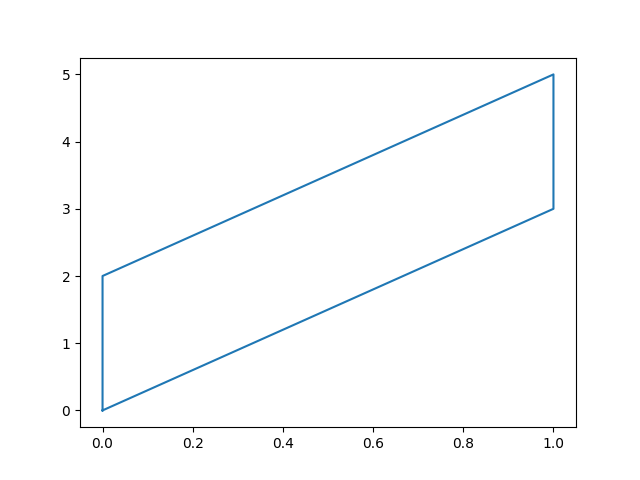
\includegraphics[scale = .5]{change_of_variables/parallelepiped-2d.png}
\caption{The image of the cube $[0,1]^2$ under $T$.}
\end{figure}

Note that the vertices are given by the image of the vertices of the hypercube. In particular, two of the vertices are precisely the columns of $T$. 

Returning to change of variables with a linear function $T$ inside of $f$, we see that $|\det T|$ gives our exchange rate inside the integral:
$$
\int_A f(x)\dx = \int_{T^{-1}(A)} f(T(x)) |\det T| \dx.
$$
More generally, if the function $g$ is nonlinear, then we must use an instantaneous exchange rate. This is obtained by linearizing $g$ at each point $x$, and computing the volume exchange rate for the linearization; i.e., $|\det Dg(x)|$. 
This result takes a measure theoretic treatment to prove generally. But this is the basic intuition. 

Also, a concrete example with a density function would be nice. So you can see how the map is sort of redistributing the mass in the density function, and how the determinant term helps 

\section{High dimensional spaces}
We often work in high dimensional spaces. Many datasets have 10 or more features. MNIST data has 728 dimensions. A high resolution image has a million dimensions. If you're working with a kernel machine, even if your data has relatively low dimensionality, it's embedded in a high dimensional space. We develop intuition in 2 and 3 dimensions. But our basic mental picture fails in serious ways to generalize in higher dimensions, where properties are counterintuitive, and sometimes quite bizarre at first sight. The purpose of this discussion is to help build intuition about high dimensional spaces so you can be a better data scientist, ML practitioner, or engineer. Also, understanding the basic geometric properties of high dimensional spaces lays the foundation for better understanding statistical properties in high dimensional spaces. 

\subsection{Volume of $d$-ball}
The ball of radius $r$ in $\R^d$ is given by
$$
B_r := \{ x\in \R^d: \|x\| \leq r\}.
$$
The volume of the ball in $d$ dimensions is obtained by integration. There are a few different ways of doing this, some pretty clever.\footnote{I was tempted to put in the version that uses the Gaussian integral, since we solved that in the CoV section. But it makes an assumption about a proportionality relationship with the surface area of high dimensional spheres that isn't obvious. And I didn't want to have to prove. And integrating this stuff out isn't really the point of these notes. So, I took the lazy route of just giving a high level idea of the brute force approach, but skipping the details because they're tedious and don't advance the objective of these notes.} But the brute force way is to just integrate in $d$ dimensions analogous to how you've done it in 3. Set up the integral you want to solve in cartesian coordinates.
$$
\int_{B_r} \dx_1\cdots \dx_d.
$$
Do a change of variables to spherical coordinates. (Hyper)-spherical coordinates in $d$ dimensions are defined analogous to the 3d case, and you can look up the conversion and wrap your head around how it works. At the end of the day, you solve the integral
$$
\int r^{d-1} \sin^{d-2}(\phi_1)\cdots\sin(\phi_{d-1}) d\phi_{d-1}\cdots d\phi_{1} dr,
$$
where I've omitted the domain because I'm lazy. But it's a product of intervals. So, a high dimensional rectangle. You chug through this integral and you get that the volume of the $d$ ball of radius $r$ is given by
\begin{equation} \label{eq:vol-of-ball}
V_d(r) = \frac{\pi^{d/2}r^d}{\Gamma(\frac{d}{2} + 1)}. 
\end{equation}
Just think of the Gamma function as an extension of the factorial to non integer values. 
Figure \ref{fig:volumes-of-balls}, taken from wikipedia, plots the volume of a few different balls as the dimension increases. Note that the volume of a ball plummets to zero as $d\to\infty$. For bigger radii, the volume will be a lot bigger in lower dimensions, but no matter what, the volume of any ball goes to zero as $d\to \infty$. That's freaking weird. 
\begin{figure}[h]
     \centering
     \begin{subfigure}[b]{0.4\textwidth}
         \centering
         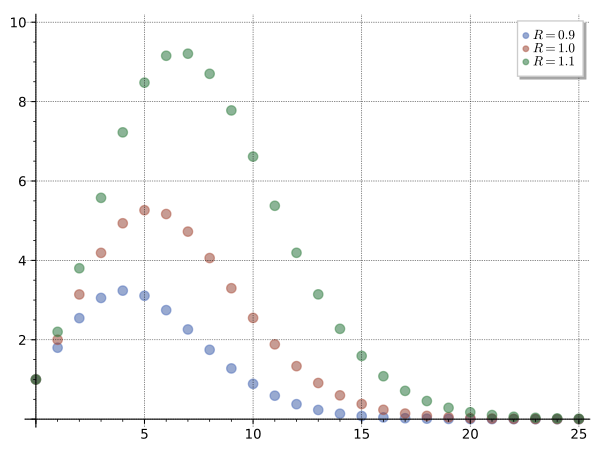
\includegraphics[width=\textwidth]{high_dimensional_space/Volumes_of_unit_balls.png}
         \caption{}
     \end{subfigure}
     \begin{subfigure}[b]{0.4\textwidth}
         \centering
         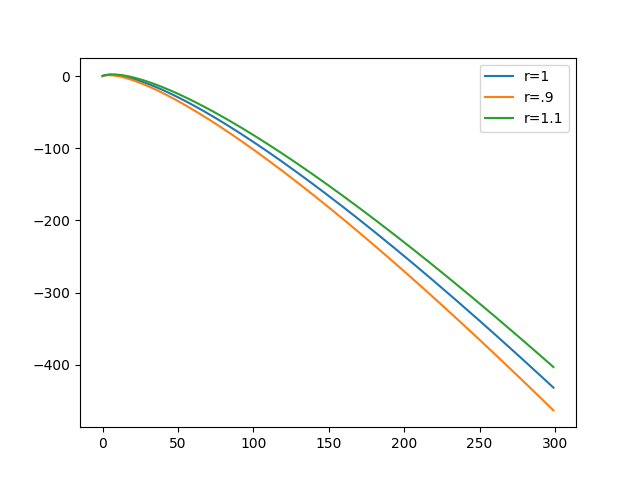
\includegraphics[width=\textwidth]{high_dimensional_space/Volumes_of_unit_balls_log.png}
         \caption{}
         \label{fig:three sin x}
     \end{subfigure}
        \caption{Volume of unit ball as a function of the dimension. (a) is the standard plot, taken from Wikipedia (b) plots the log of the volume vs dimension.}
        \label{fig:volumes-of-balls}
\end{figure}


%Good way to approach this: Don't state the title about your intuition is wrong. Just ask to speculate about some properties? I don't know. Maybe start by focusing on 1 ball. Consider what volume does as dimension increases. It's bizarre that it goes to zero. Then consider $r>1$. And note that no matter how big the radius of the ball, eventually it goes to zero. This has to do with Euclidean topology. If you consider other $Lp$ balls, I don't think they do this. 



\subsection{Balls and Cubes}
Consider a ball of radius 1/2 inscribed inside a cube of width 1. e.g., 2d example. The ball always touches the surface of the cube. As $d$ increases, the volume of the cube stays one. But the volume of the sphere inside goes to zero (quickly!). As another example, consider a ball of radius 1 and cube of width 1. Draw in 2d. The cube is contained well within the ball. But when we go to 3 dimensions, the gap closes a bit. The corner of the cube is at $\sqrt{d/2^2} = 1/2\sqrt{d}$. At $d=4$ the corners of the unit cube touch the surface of the ball of radius 1. For $d>5$, the corners poke through the surface. Moreover, there are $2^d$ vertices poking through. 


\subsection{Most of the mass is near the equator}
%\begin{figure} \label{fig:volumes-of-balls}
%\centering
%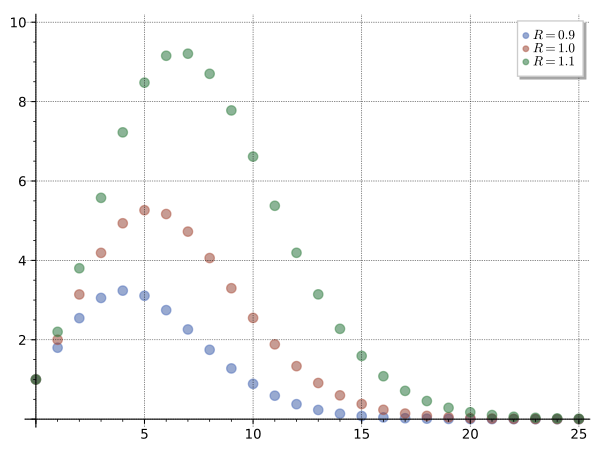
\includegraphics[scale = .5]{high_dimensional_space/Volumes_of_unit_balls.png}
%\caption{Volumes of $d$ balls.}
%\end{figure}
See section 1.2.3 of the CMU book chapter on geometry of high dimensional spaces. 

Consider a small slice through the ball near some equator. That is, consider the portion of the ball that lies "above" the plane where $x_1 = \epsilon$. One can show that very little of the volume of the sphere lies in this region. This is accomplished by simply integrating (and using a few approximations). Add this if I have time. But I'm not sure it's worth the trouble of working through the integration. the end result is the following lemma. 
\begin{lemma}
For any $c>0$, the volume of the hemisphere above the plane $x_1 = \frac{c}{\sqrt{d-1}}$ is less than $\frac{2}{c}e^{-c^2/2}$. 
\end{lemma}
Intuitively, I think this makes a lot of sense. You're fixing a plane by setting $x_1=0$ and considering a $\epsilon$ padding of that plane, and considering how much mass is in that padded region. While it's true that $\epsilon$ is small, by considering a plane, you're considering an $d-1$ dimensional set. When you move in the orthogonal direction, you only have 1 dimension to move in. In some sense, this dimension can't contain a lot of volume. Most of the volume is contained near the plane. 

You can get some intuition for this by going from 2 dimensions to 3 dimensions. If you fix a diametric plane in 2 dimensions, then moving orthogonal to the plane you capture a lot of volume. Now do the same thing in three dimensions. More of the volume is contained near the equatorial plane. As the dimension increases, more and more of the volume is contained near $d-1$ dimensional equatorial hyperplane. 

While the idea that most of the mass is near the equator, its implication in practice is almost stupidly obvious. Suppose you draw a uniform random sample from the unit ball. Then with high probability, all of the coordinates are going to be small. This makes sense when you think of the fact that the norm of the sample must be contained near within a radius of $1$. If any one of the components is close to 1, then the others have to be really, really tiny. Another way to think about it, suppose that $x_i = $ big, for some coordinate $i$. This means that the other coordinates must all be contained in a very small $d-1$ dimensional ball. But the product of a tiny $d-1$ dimensional ball with, even the entire diameter of the circle, is going to have really small volume. So, that's not going to happen. 

\subsection{Most of the volume is near the surface}
(Copied from cmu book.) By \eqref{eq:vol-of-ball}, the ratio of the volume of a sphere of radius $1-\eps$ to the volume of a unit sphere in $d$ dimensions is $
(1-\eps)^d.$
This is shown in Figure \ref{fig:vol-near-surf}. 
The higher the dimension, the more the volume is concentrated on the surface of the sphere. This basically follows from the fact that the higher $d$, the more $x^d$ looks flat below 1 and like a wall straight up at 1. 
\begin{figure} \label{fig:vol-near-surf}
\centering
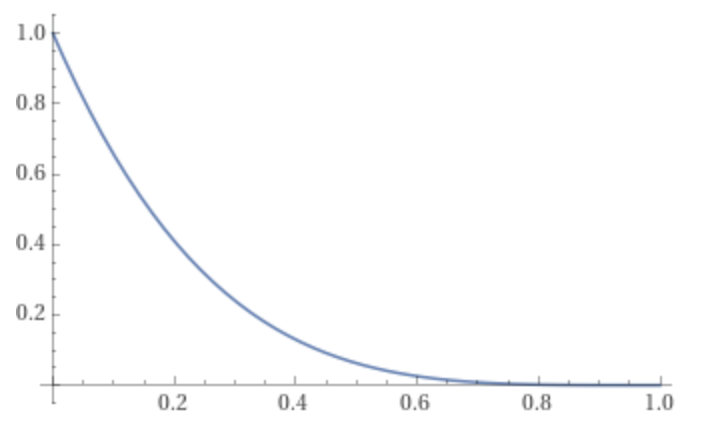
\includegraphics[scale = .5]{high_dimensional_space/vol-near-surf.png}
\caption{Volume near surface of sphere.}
\end{figure}

\subsection{High dimensional cubes}
The fact that most of the volume of a high dimensional ball is near the surface is a little more transparent when you look at hypercubes. (Which, I'm going to call a ball, even though by ball here, we really do only mean L2 ball, which is an important distinction. The volume near the surface property is probably true for any convex body?) 
Consider a unit cube, and the volume outside the inner cube with side length $1-\epsilon$. Draw this out for 1, 2, and 3d. The volume of the inner region diminishes as $(1-\eps)^d$. (See other notes on this for a compelling presentation.) 


\subsection{Distances between randomly sampled points}
Suppose you sample two points uniformly at random from the unit ball. How far apart will they be? Show demo. Answer is that even though the volume of the ball is going to zero, the distance between randomly sampled points converges to a constant. State a general result about distance between furthest and closes points, for iid case. (Technically, this won't cover the ball case. But it tells us something.) 

Question: What does this mean about things like knn? Under reasonably general conditions, you can show that as the dimension grows large, the distinction between nearest and furthest point vanishes. An example of this is the following result. 
\begin{theorem}
Suppose that $X_n\in \R^d$ is composed of $d$ iid random variables and that for some $k\geq 1$, $\lim_{d\to\infty} \frac{\|X_d\|_k}{\E \|X_d\|_k} = 0$. Then 
$$
\frac{D_{max, d}^k - D_{min, d}^k}{D_{min, d}^k} \to_{p} 0 \quad as \quad d\to \infty,
$$
where $\to_p$ indicates convergence in probability to the point mass on zero. 
\end{theorem}

Example: Sampling points from the $d$-cube. (TODO: Add computational example. TODO: Is there an interesting two-class classification version of this? Like, can you distinguish between points on opposite sides of a hypercube? Probably best to just look at that paper. TODO: If I don't have time to do this now, then that's OK. Maybe this is good fodder for discussion. When does this tell us about when knn breaks down? How does this impact things like neural networks operating in high dimensional spaces?)  

Moral: You need to be careful about the meaning of distance metrics and similarity in high dimensions. 

\subsection{Digression: Lp balls}
Question: We've implicitly looked at l2 and l-infty balls. You can consider similar properties for other lp balls. Note paper about surprising properties of distances. Add reference. Moral of that paper: Can consider fractional distances, and these tend to be a little more meaningful. 

\subsection{Discussion}
Mention things like, is data really usually high dimensional. No. usually does something like live in a lower dimensional manifold. Touch on importance of dimensionality reduction for being able to say meaningful things about data in something like knn. Touch on PCA and isomap. 

Mention that sometimes you intentionally move up to higher dimensions. Usually for kernel methods. This allows you to do things like linearly separate classes of data. Mention Cover's theorem. 

This also makes me wonder about SVMs in high dimensions (not even kernel SVM). Like, if you've got a two-class data set, and you're trying to find the largest margin linear separating hyperplane, this is ultimately a distance problem in a high dimensional space. I've always taken for granted that my intuition from 3 dimensions implies that there are no sticky issues when doing this. But is that true? 


%Outline:
%- High dimensional balls. Definition. Volume of unit ball? (This is a TODO. Would like a relatively clean derivation of this that I can follow fully.) Surface area? (Maybe just state this, not derive, if we're already deriving volume.) Distance between two points sampled from ball? Maybe just show this with an example. Counterintuitive that the volume is going to zero, but the distance between points stays constant? (Is that true?) Most of the volume is at the equator. Derive. Discuss: In 3d, this property seems counterintuitive when you're visualizing a high dimensional ball as just sort of a higher dimensional version of a 3-ball. But it makes more sense when you realize that it's a totally different object. For a 3 ball, if most of the mass is at the equator, then you would think that if you take a different (say ``orthogonal'') equator, then most of the mass can't be there too. Because it's already in the other equator. The point of this example is to show you that your intuition is broken. You can't just extend your intuition from 3 balls here. n-balls are weird objects. Next property: - Intersection of equators? (Show that two strips around different equators have a lot of mass in common. Not sure how to show this.) Most of the volume is in a shell near the surface. Computation example: Sample points iid uniform from the $n$ ball. What's the distance between them? As $n$ grows large, all points tend to be a constant distant apart (experimentally). Hence, the volume of the $n$ ball goes to zero, but points sampled from the ball all tend to be a constant distant apart. High dimensional space is weird. We'll see shortly that this constant distance property has important implications for ML/data science. 
%- High dimensional cubes. Volume of the 1cube stays constant. Unit cube and 1/2 inscribed ball. Volume of the inscribed ball goes to zero. Unit cube and 1-ball. As dimension increases, the corners of the unit cube poke out of the 1ball, and take up all the volume. Again, the volume of the ball goes to zero. But the volume of the cube stays constant. Maybe note that here you can easily see that most of the volume of the ball is again at the surface of the cube. 
%- Comment on the fact that when you take an epsilon ball about a point in $\R^d$ in proofs, you're actually doing this funky thing. 
%- What does all of this have to say about classification in high dimensions? In particular, what does it have to say about KNN classification? Reference: 
%%https://minds.wisconsin.edu/bitstream/handle/1793/60174/TR1377.pdf?sequence=1&ref=https://githubhelp.com. 
%TODO: Briefly look over this and the surprising results about distance metrics in high dimensions. State a summarized version of their theorem that points all about equidistant in high dimensional space. Relate this to an actual sampling and classification problem, so you can see why knn in high dimensions would be problematic. Don't spend a ton more time on this. 
%- A few other incidental questions and issues to bring up. How often does high dimensional data really arise? I mean, often, yes. But is it genuinely high dimensional, or does it live in a lower dimensional space? This brings up the importance of dimensionality reduction techniques for certain types of data processing. PCA is one method, but it only really works if the data lives in a linear subspace. You have to consider your data assumptions. If your data lives on a smooth manifold, then you can use something like isomap. What are other structures the data might have? clusters? spheres in spheres? Like, what are reasonable data topologies you might expect, and what are good ways to ``reduce'' the dimension in order to do analysis. This isn't always simple. e.g., if the data lives on $S^2$ sphere, then how do you reduce it to 1 or two dimensions? This is a cartographers problem. And no matter what you do, you're going to break some of the topological properties. Something you can do to fully capture the relationships mapping to 2d is to produce 2 different maps that slice the sphere along different lines. Then the manifold distance relationships on both are true, even though they seem to conflict somewhat. Something else that's worth considering is if you want to just construct something like a graph that you'll use for label propagation, then you can do it using similarity in high dimensions, under the assumption that the data lives on a reasonably low dimensional manifold. That will actually preserve connections around things like spheres. 
%- Kernel methods. Sometimes we intentionally lift data to a higher dimensional space. The intrinsic dimension of the data is the same as the original dimension. (Footnote to theorem reference.) But in high dimensions, binary data can become linearly separable. There is also kernel PCA,, which doesn't rely on labels. But I'm not sure I actually understand the value of kernel PCA other than understanding what your kernel machine is doing. It's true that it can do things like make concentric rings look linearly separable. But this isn't really well understood. (Possible open research question?) 
%- Something else to integrate: The n-ball above is the Euclidean ball. The hypercube is the Linfty ball. Are certain Lp norms better for certain purposes? This paper is useful: https://bib.dbvis.de/uploadedFiles/155.pdf


\section{High Dimensional Gaussian }
Random variables in high dimensional spaces can behave in counterintuitive ways. We typically develop intuition in low dimensions, but don't realize which aspects of our intuition fail to extend to high dimensional spaces. A good place to start building better intuition is looking at the properties of high-dimensional Gaussian random variables. The main property of high dimensional Gaussians that you'll hear cited is that most of the mass is concentrated around the surface of a sphere. The reason for this bizarre effect has to do with more basic properties of high dimensional geometry than anything else. A high-dimensional ball has most of its mass concentrated on the surface of a sphere. We'll begin by briefly considering properties of high-dimensional spheres and hypercubes, and then characterize the high dimensional Gaussian. 

\subsection{Radial density of Gaussian}
Suppose $x\in \R^d$ is sampled from an isotropic Gaussian. We would like to understand the density of $r= \sqrt{\sum_{i=1}^d x_i}$. To this end, first note that the random variable $r$ can be viewed as 
$$
r = \sqrt{w} 
$$
where $w$ is a $\chi^2$ distribution with $d$ degrees of freedom having density
$$
f_w(w) = cw^{\frac{d}{2} - 1}e^{-\frac{d}{2}},
$$
and $c$ is a proportionality constant that I'm ignorning.
Applying the change of variables expression \eqref{eq:pushforwardY}, we can compute the density of $r$. We have $h(r) = g^{-1}(r) = r^2$ and $Dh = 2r$. Subbing this in we get
$$
f_r(r) = cr^{d - 2}e^{-\frac{r^2}{2}}r = cr^{d-1}e^{-\frac{r^2}{2}}, 
$$
where we absorb stuff into the constant. 
We would like to characterize where most of the mass of $f_r(r)$ lies. A plot of $f_r(r)$ for various values of $d$ is shown in Figure ??. In general, the plots suggest that $f_r(r)$ is log concave, and most of the mass is concentrated in a band that increases roughly as $\sqrt{d-1}$. Our plan of attack will be 
\begin{enumerate}
 \item Take the log of the density, so we hopefully deal with a concave function
 \item Consider an interval $I$ of width $2d$ about the maximum of the function. We'll try and characterize the amount of mass in this interval. 
 \item Construct a second order approximation of the function. In particular, construct an upper bound on the function and then use this to bound the amount of mass outside of the interval. 
 \item Because we've been cavalier with the proportionality constant, we don't know what the total mass of $f$ is. (It's not a probability density.) We'll come up with a lower bound on the total mass of $f_r$ and use that to estimate the fraction of mass in the interval $I$. 
 \item Continuing with the previous point, let $M_{\bar I}$ be the mass outside the interval $I$ and let $TM$ denote the total mass. We are interested in estimating
 $$
 \mbox{quantity of interest } = \frac{M_{\bar I}}{TM}.
 $$
We'll compute an upper bound on $M_{\bar I}$ and a lower bound on $TM$, to get an upper bound estimate on the quantity of interest. If we can say that QOI is small, then it means that most off the mass lies in the interval $I$. Through all of this, we'll make our estimate depend on $c$, the width parameter of $I$, so that we'll be able to estimate the amount of mass in $I$ as a function of width. 
\end{enumerate}

We now proceed along those lines. 
Disregarding the proportionality constant, let 
$$
g(r) := r^{d - 2}e^{-\frac{r^2}{2}}r = cr^{d-1}e^{-\frac{r^2}{2}} \quad \mbox{ and } \quad f(r) = \log g(r) = (d-1) \log(r) - \frac{r^2}{2}.
$$
Note that 
$$
f'(r) = \frac{d-1}{r} - r \quad \mbox{ and } f''(r) = \frac{-(d-1)}{r^2} - 1 \leq -1.
$$
The second inequality implies that $f(r)$ is concave (and $g(r)$ log concave). Hence, solving for $f'(r) = 0$, we see that $f$ is maximized at $\sqrt{d-1}$. Applying Taylor's theorem about $r=\sqrt{d-1}$ and we have
\begin{align}
\label{eq:gauss-sphere-f-taylor}
f(r) & = f(\sqrt{d-1}) + \underbrace{f'(\sqrt{d-1})}_{=0}(r-\sqrt{d-1}) + \frac{1}{2}f''(\zeta)(r-\sqrt{d-1})^2\\ 
& \leq f(\sqrt{d-1}) - \frac{1}{2}(r-\sqrt{d-1})^2
\end{align}
for some $\zeta$ between $r$ and $\sqrt{d-1}$. In the first line, we have applied a form of Taylor's theorem where we explicitly handle the remainder. (This can be found on Wikipedia, and would be a good topic for future notes. On the board, maybe set this part up by first stating the standard form of Taylor's theorem. Then backtrack and note that this this other convenient form that allows us to explicitly handle the remainder. Though, to be honest, could you just use the standard form?) In the last line, we apply the fact that $f''(\zeta) \leq -1$. 
By the definition of $f$, this gives
\begin{align}
g(r) & = \exp(f(r)) \\
& \leq \exp(f(\sqrt{d-1}) - \frac{1}{2}(r-\sqrt{d-1})^2 )\\
&  = g(\sqrt{d-1})\exp(-\frac{1}{2}(r-\sqrt{d-1})^2 ).
\end{align}
As desired, we have a simple ``quadratic'' estimator on $g$. Let $r_d = \sqrt{d-1}$, because I'm tired of writing this, and for a constant $c>0$ consider the interval 
$$
I = \{r_d - c, r_d+c\}. 
$$
Let's try to bound the mass outside this interval using our quadratic overestimator. 
\begin{align}
\int_{r\not\in I} g(r)\dr & \leq \int_0^{r_d - c} g(\sqrt{d-1})\exp(-\frac{1}{2}(r-\sqrt{d-1})^2 ) \dr + \int _{r_d+c}^{\infty} g(\sqrt{d-1})\exp(-\frac{1}{2}(r-\sqrt{d-1})^2 )\dr\\
& \leq 2g(\sqrt{d-1})\int _{r_d+c}^{\infty} \exp(-\frac{1}{2}(r-\sqrt{d-1})^2 )\dr\\
& = 2g(\sqrt{d-1})\int _{c}^{\infty} \exp(-y^2/2)\dy\\
& \leq 2g(\sqrt{d-1}) \int _{c}^{\infty} \frac{y}{c}\exp(-y^2/2)\dy\\
& = \frac{2}{c}g(\sqrt{d-1})\exp(-c^2/2).
\end{align}
In the first line, we use the upper bound on $g$. In the second line, we use the fact that the upper bound is symmetric about $r_d$, so integrating over the right half interval is at least as large as the left interval (which is truncated at zero). 
In the fourth line we use the fact that $y\c > 1$ in the interval of integration. (We do this with a change of variables in mind.) In the last line, we apply change of variables. TODO: Actually check the application of COV in the last step. This will be our estimate on $M_{\bar I}$. 

Now, let's come up with a lower bound on the total mass. We'll do this by considering only the mass of $g(r)$ in the subinterval $[r_d-c, r_d]$. For $r$ in this subinterval, we have $f''(r) \leq -2$. This is confirmed by noting that $f''$, as explicitly computed above, is monotonically increasing for $r>0$, and then evaluating $f''$ at the left endpoint of the interval. Applying \eqref{eq:gauss-sphere-f-taylor}, we have 
$$
f(r) \geq f(\sqrt{d-1}) - (r-\sqrt{d-1})^2 \geq f(\sqrt{d-1}) - \frac{c^2}{4}
$$
for $r$ in the designated subinterval. 
Equivalently, this gives
$$
g(r) \geq g(\sqrt{d-1})\exp(- \frac{c^2}{4}). 
$$
Applying this (and noting that the bound has no dependence on $r$), we see that the total mass is at least
$$
\int_{r_d - c}^{r_d} g(r)\dr  \geq cg(\sqrt{d-1})\exp(- \frac{c^2}{4}).
$$
Finally, we see that
 $$
\mbox{QOI} = \frac{M_{\bar I}}{TM} \leq \frac{\frac{2}{c}g(\sqrt{d-1})\exp(-\frac{c^2}{2})}{cg(\sqrt{d-1})\exp(- \frac{c^2}{4})} = \frac{2}{c^2}\exp(- \frac{c^2}{4}).
 $$
 This proves the following lemma (wording directly copied from Blume/Kannan/Hopcroft book). 
 \begin{lemma}
 For a $d$-dimensional spherical Gaussian of variance 1, all but $\frac{2}{c^2}\exp(- \frac{c^2}{4})$ fraction of its mass is within the annulus $\sqrt{d-1} - c \leq r \leq \sqrt{d-1} + c$. 
 \end{lemma}
 Some concrete implications: Independent of $d$, $.99$ fraction of the mass is contained in the annulus with $c = 3.38$. and $.999$ fraction of the mass is contained in the annulus with $c=4.32$. 
 
 \vspace{1em}
\noindent \textbf{Can we do better?} This estimate holds for $d$ arbitrarily large. One may wonder if this is a conservative estimate. Perhaps the mass actually concentrates onto an arbitrarily narrow annulus as $d\to \infty$? My experimentation suggests that this is not the case. I think that the width of the high mass region is genuinely ``constant'' independent of $d$. 
 
 Example: To generate samples from a traditional VAE, one draws samples from a unit gaussian and then passes these through a neural network. For moderately high dimensional latent space, this means that the samples are roughly drawn from the surface of a unit sphere. A question one might ask is: How does this affect interpolation? One of the most useful properties of a VAE is the ability to interpolate in latent space. But, if you draw two samples from a high dimensional gaussian and consider the euclidean ``straight line'' interpolation between them, are you passing through regions where there is very little mass, and so you probably have few samples? Or do your interpolations tend to stay close to the surface of the sphere as well? Is there a better way/different geometry to interpolate rather than straight lines?
 
 Example: TODO: Give an information theory example, like from the Shannon paper about communication in the presence of noise?

TODO: Show some simulation examples. 


%Outline:
%- Question: If you sample from a high dimensional gaussian, can you say roughly where it will lie radially?
%- Idea: the density has the most mass near the origin. But there's almost no volume here. The probability of drawing a sample from a set $A$ is $\int_A f_X(x)\dx$. There's almost no volume here. So the probability of drawing a sample will be small. Eventually, when you get far out, there's tons of volume, but the density drops off. So, again, unlikely to get samples out there. Is there a happy medium where most of the mass lies? (Think of it like, high density in the middle, but no volume, so low overall mass. The probability of sampling from a given region is given by the mass of the region. It's a weird but cool way to think about things.) 
%- Derive density in terms of r
%- Show that most of the mass lies near the surface of a sphere. (TODO: There is one step in this proof that I'm not following. Go back and look this up.) 
%- Show a plot of the density we derived. Show that it clearly concentrates near where we said it would. 
%- Draw some samples from a high dimensional gaussian.  
%- Comments:
%  - we think that samples would lie near the mode. But they don't. Also, a gaussian is log concave. So we sort of think that samples should roughly lie in a convex set. But they really don't. Which is important, I imagine, because if you think a set is convex but it's not, you can get yourself into some real trouble, especially if you're in optimization land. 
%  - Example: Information theory and perturbations of high dimensional signals. 

%\begin{itemize}
%  \item introduce idea of high dimensional Gaussian characterization. Basically, there is a lot more volume on the surface of a sphere in high dimensions. But Gaussian tail is exponential. At some point, drop off in probability with overwhelm increase in volume due to space. So, where is mass most concentrated?
%  \item Review change of variables formula (May need to add some notes just on this. Introduce it. Give some intuition for what it means. Give some examples in probability. (Just illustrate it on a few different distributions.) Give example with law of the unconscious statistician. Give example deriving polar change of coordinates. Give example with reparameterization trick?) 
%  \item Use change of variables to derive distribution of radius r of a high dimensional gaussian (start from chi squared)
%  \item Use this form to derive estimate on where most of the mass lies radially
%  \item Show analytically where the pdf of a high dimensional normal lies. 
%  \item Show in simulation where it lies. 
%  \item Review takeaways: Basically, this helps to build better intuition about how high dimensional random variables/probability works. Also, incidentally, useful in information theory. Also, cite paper about using high dimensional gaussians to characterize loss surface of neural networks. 
%\end{itemize}


%- The mass of a high dimensional  ($d$-dim) gaussian is concentrated on the surface of a sphere of radius $\sqrt{d-1}$. 
%- The question we're wondering about is: If you pick a random draw from a high dimensional gaussian, can you estimate the radius? (Why are we asking this? I'm not certain, actually. It does come up. When? Information theory. Also, do you model high dimensional data as being drawn from a Gaussian? I'm not sure. But I'm certain this comes up a lot. So I should be able to find some compelling motivation later.) 
%- The central thing I want to show is that the mass of a high dimensional gaussian is concentrated about the surface of a sphere. 
%- Having motivated that we want to understand where most of the mass of a high dimensional gaussian lies, and in particular, the length of a random gaussian vector, we can start by building intuition in 1-2 dimensions. Here, most of the mass is clearly concentrated about the origin. A 3d Gaussian is harder to visualize. Intuition suggests that this pattern continues into higher dimensions. But it doesn't. 
%- To see this, show some simulations of a high dimensional Gaussian, and where it concentrates radially. 
%- The reason for this "concentration of mass" in an annulus is that, despite the pdf being large near the center of a sphere, there is a relatively small amount of volume there. But there is tons of volume in larger outer shells. Here, we have the competing factors of the amount of volume increasing exponentially radially outwards (so we have more space to integrate over), and the gaussian distribution decaying squared-exponentially radially. So, there's a happy medium where it settles. 
%- Before considering high dimensional Gaussians, let's consider geometry of high dimensional spheres. Build intuition that if you have a concrete rod, circle, and sphere, more and more of the mass is concentrated in the outer shell of width epsilon. This seems clear if you consider the three objects and then ask which contains the most mass in its outer "shell". This pattern continues into higher dimensions. 
%- Spend some time developing intuition for high dimensional balls. key points - Most of mass of the unit ball is on the surface. Weird. Interior is nearly empty. - Comparison of high dimensional cube vs sphere. - Discussion about most of the mass lying near the equator. 
%- From here, transition back to high dimensional gaussians. Derive the density function. Do this using change of variables from a chi2 distribution. Then, using the density function, derive the amount of mass contained in an annulus using p21 from these notes https://www.cs.cmu.edu/~venkatg/teaching/CStheory-infoage/chap1-high-dim-space.pdf.



Todos
\begin{itemize}
  \item Geometry of high dimensional spheres and cubes
  \item Gaussian in high dimensions (characterize. Maybe there's a reference in one of those old papers about characterizing local minima of neural networks.) 
  \item Law of unconscious statistician (do this and polar and Gaussian constant as applications of change of variables. Then reference all kinds of generative models.) 
  \item Brachistochrone problem
  \item integration by parts and connections with FTC.
  \item review of IFT and connection to inverse function theorem? And connections to FTC?
\end{itemize}

%\section{PCA}
%\begin{itemize}
%  \item Computationally, PCA is just the eigendecomposition of the sample covariance matrix. Review the sample covariance matrix. Why do we use this? (We just do?) 
%  \item Two common ways of looking at this/interpreting the meaning of the eigenvectors/deriving that this eigendecomposition is what you're looking for. 
%  \item 1. Compute a unit vector d such that the projection of data points onto d has maximal variance. 
%  \item 2. You want a lower dimensional subspace, of some fixed dimension $d$ such that the projection of the data onto the subspace has minimal reconstruction error. 
%  \item 3. Say your data is represented as a matrix $X$ (assume centered data). Compute the best low rank approximation to $X$
%  \item Comment: Why are 1 and 2 equivalent? Think of projecting a point onto a subspace. Consider the triangle between the point, the projection, and the origin. The data is fixed. You can change the projection subspace, which implicitly changes the other two legs of the triangle. Minimizing the reconstruction leg is equivalent to maximizing the variance leg. That's one data point. When you sum these together, the same property should hopefully still hold. 
%  \item Walk through each of these. For the first one, you have to set things up by reviewing the KKT conditions. All that's really needed for this is to define the dual function. Show the lower bound property. Then state the KKT conditions for convex problems. Then show that a solution to these conditions implies optimality for a convex problem. (As a sidenote, I think it would be really interesting to work through some problems where the lagrange multipliers have a physical interpretation. Like, force onto a wall. Or an electrical circuit. Or an economics example.) 
%  \item It's relatively easy to show the maximum variance perspective from here. 
%  \item Then show the projection perspective. 
%  \item I think the low rank approximation perspective is really easy. The best low rank approximation is just the SVD. And the definition of the SVD is basically the eigendecomposition of $XX^T$. (Actually, this perspective makes it obvious why you can solve a different system, depending on whether $d$ or $N$ is larger. You just solve for the right or left singular vectors. 
%  \item Then you have kernel PCA. What do I want to know about this? Start by reviewing what we're trying to do here. Send our data into high dimensional feature space. Then figure out the direction of maximal variance (need it exist?!) And then look at the corresponding latent codes as represented via the canonical basis in $R^n$? Hm. That's kind of weird. 
%\end{itemize}



\bibliographystyle{alpha}
\bibliography{sample}

\end{document}